% !TeX encoding = UTF-8
% !TeX program = pdflatex
% !TeX spellcheck = en_US

\documentclass[LaM,binding=0.6cm]{./packages/sapthesis/sapthesis}

\usepackage{microtype}
\usepackage{amssymb}
\usepackage{amsmath}
% Norm Command
\newcommand{\norm}[1]{\left\lVert#1\right\rVert}

\usepackage{hyperref}
\hypersetup{pdftitle={Robustness of Deep Neural Networks Using Trainable Activation Functions},pdfauthor={Federico Peconi}}

% Remove in a normal thesis
\usepackage{lipsum}
\usepackage{curve2e}
\usepackage{algpseudocode}
\definecolor{gray}{gray}{0.4}
\newcommand{\bs}{\textbackslash}

% Commands for the titlepage
\title{Robustness Of Deep Neural Networks \\Using Trainable Activation Functions}
\author{Federico Peconi}
\IDnumber{1823570}
\course{Computer Science}
\courseorganizer{Computer Science - Informatica LM-18}
\AcademicYear{2019/2020}
\copyyear{2020}
\advisor{Prof. Simone Scardapane}
%\advisor{Dr. Nome Cognome}
%\coadvisor{Dr. Nome Cognome}
\authoremail{peconi.1823570@studenti.uniroma1.it}

\examdate{Something October 2020}
\examiner{Prof. Nome Cognome}
\examiner{Prof. Nome Cognome}
\examiner{Dr. Nome Cognome}
\versiondate{\today}



\begin{document}

\frontmatter

\maketitle
\dedication{Dedicated to\\ Donald Knuth}

\begin{abstract}
This document is an example which shows the main features of
the \LaTeXe\ class \texttt{sapthesis.cls} developed by 
with the help of GuIT (Gruppo Utilizzatori Italiani di \TeX).
\end{abstract}

\begin{acknowledgments}
Ho deciso di scrivere i ringraziamenti in italiano
per dimostrare la mia gratitudine verso i membri
del GuIT, il Gruppo Utilizzatori Italiani di \TeX, e, in particolare,
verso il prof. Enrico Gregorio.
\end{acknowledgments}

\tableofcontents

% Do not use the starred version of the chapter command!
%\chapter{Capitolo non numerato}

\mainmatter

\chapter{Introduction}

    \section{Intriguing Properties of Neural Networks}

        Here we informally state the problem of adversarial attacks in ML models 
        especially wrt to Neural Networks.
        Why is it of fundamental importance for the progress of the field from
        both practical (nns cant yet be deployable in critical scenarios for such reasons ) 
        and theoretical (Madry arguments around interpertability and robustness)
        perspectives

        %Recent work has shown that state-of-the-art classifiers are quite brittle, in the sense that a small adversarial change of an originally with high confidence correctly classified input 
        %leads to a wrong classification again with high confidence. 
        %This raises concerns that such classifiers are vulnerable to attacks and calls into question their usage in safety-critical systems.
%
        %Why might we prefer to use the adversarial risk instead of the traditional risk? If we are truly operating in an adversarial environment, where an adversary is capable of 
        %manipulating the input with full knowledge of the classifier, then this would provide a more accurate estimate of the expected performance of a classifier. 
        %This may seem unlikely in practice, but several classification tasks (especially those relating to computer security) such as spam classification, malware detection, 
        %network intrusion detection, etc, are genuinely adversarial, where attackers have an direct incentive to fool a classifier. 
        %Or even if we don’t expect the evironment to always be adversarial, some applications of machine learning seem to be high-stakes enough that we would like 
        %to understand the “worst case” performance of the classifier, even if this is an unlikely event; this sort of logic underlies the interest in adversarial examples in domains 
        %like autonomous driving, where for instance there has been work looking at ways that stop signs could be manipulated to intentionally fool a classifier.
%
        %However, there is also a reasonable case to be made that we might prefer empirical adversarial risk over traditional empirical risk, even if we ultimately want to minimize the 
        %traditional risk. The reason for this is that it is very difficult to actually draw samples i.i.d. from the true underlying distribution. 
        %Instead, any procedure we use to collect data is an empirical attempt at accessing the true underlying distribution, and may ignore certain dimensions, especially if these appear “obvious” 
        %to humans. This is hopefully somewhat obvious even on the previous image classification example. 
        %There has been a lot of recent claims that algorithms have “surpassed human performance” on image classification, using classifiers like the one we saw as an example. 
        %But, as the above example illustrates, algorithms are nowhere near human performance, if they cannot even recognize that an image that looks exactly the same, 
        %by any visual definition, as the original image, in fact belongs to the same class. Some may argue that these cases “shouldn’t count” because they were specifically designed to fool 
        %the algorithm in question, and may not correspond to an image that will ever be viewed in pratice, but much simpler pertrubations such as translations and rotations also can serve as 
        %adversarial examples.
%
        %The fundamental problem is that when claims are made of “human level” performance by ML systems, they really mean “human level on data generated exactly by the sampling mechanism used 
        %in this experiment.” But humans don’t do well just on one sampling distribution; humans are amazingly resilient to changes in the environment. So when people are told that machine learning 
        %algorithms “surpass human performance” (especially when conjoined, as they often are, by claims that the associated deep learning algorithms “work like the human brain”), 
        %it often leads to the implicit assumption that the algorithms will also be similarly resilient. But they are not; deep learning algorithms are incredibly brittle, 
        %and adversarial examples lay this fact bare, in a very obvious and intuitive manner. Put another way, can’t we at least agree to cool it on the “human level”, and “works 
        %like the human brain” talk for systems that are as confidence that the first image is a pig as as they are that the second image is an airplane?



    \section{Smooth Activation Functions and Robustness}

        Recently a link has been proposed between activation functions and the robustness of
        Neural Networks (Smooth Adversarial Training). In particular, authors showed how they managed
        to improve the robustness by replacing the traditional Rectified Linear Units activation functions
        with smoother alternatives such as ELUs, SWISH, PReLUs
        
        Building up from this result we thought we could find benefits by laveraging recently proposed smooth
        trainable activation functions called Kernel Based Activation Functions (Scardapane et al.), 
        which already showed great results in standard tasks, in the context of adversarial attacks.
        
    \section{Structure of the Thesis}

    This paper studies the robustness of defenses to adversarial examples. Readers familiar with the
    relevant literature and notation (Szegedy et al., 2014; Carlini  Wagner, 2017b; Madry et al. Athalye et al., 2018a) can continue with Section 3 where we describe our methodology.
    In this first part, the building blocks needed in order to understand the main arguments of the thesis are introduced. Even if, at first sight, 
    the concepts that are going to follow may appear apart, the scope of this work is to make an attempt at discovering connections that might instead lie between them.     
    For this reason, we will extensively introduce what Neural Networksis important that we cover the basicsDue to the deep and wide nature depth and the wide  
    Pointers to more appropriate and detailed resources on the topics are given throughout
    
    Description of the remaining chapters 

\part{Fundamentals}


\chapter{Neural Networks}

        Broadly speaking, the field of Machine Learning is the summa of any algorithmic methodology whose aim is to automatically find meaningful patterns inside data without
        being explicitly programmed on how to do it. Well known examples are: Decision Trees (ref.), Support Vector Machines (ref. ), Clustering (ref.),
        Neural Networks (Ref. ) and, more recently, 
        Deep Neural Networks (ref. ). During the last two decades Deep Neural Networks have gained a lot of attention for their outstanding performances in different tasks like
        image classification (ref. ImageNet, over human level), speech and audio processing(ref ).

        \section{Definition}
            
            Neural Networks (NNs) are often used in the context of Supervised Learning where the objective is to model a parametric function 
            $ f_{\theta} \colon \mathcal{X} \to \mathcal{Y}$ given $n$ input-output pairs $S = \{(x_i, y_i)_{i=1}^n\} $ with $x_i \in \mathcal{X}$ and $ y_i \in \mathcal{Y}$
            such that
            \begin{equation}
                f_{\theta} \sim f  
            \end{equation}
            where $f$ is assumed to be the real input-output distribution that we want to learn. In plain words, this means that we want to find the best set of parameters $\theta^{*}$ for the model
            such that, for any unseen input $x_{new}$ we have that $f_{\theta^*}\left(x_{new}\right)$ is as close as possible to $f\left(x_{new}\right)$

            For the sake of explanation, assume the input, which in practice can be very complex and unstructured e.g. made of: graphs, text, sounds, ecc, to be embedded in an input space  $\mathcal{X} = \mathbb{R}{^d}$.
            The simplest form of a neural network is then given by
            \begin{equation}
                \label{layer}
                f_{W, b}\left(x\right) = \sigma(Wx + b)
            \end{equation}
            where the parameters of the network are the elements of a $u \times d$ matrix $ W $ and a $u$-dimensional vector called bias. The last element $ \sigma $ applied at the end is a
            function which consists of a non-linear function acting element-wise and is the key component to introduce non linearity in NNs allowing them to model 
            highly non-linear functions. We call it \textit{activation function}. \ref{layer} can then be rewritten:
            \begin{equation}
                f_{W, b}\left(x\right) = \left[\sigma(W_1^{\intercal} x + b_1), \sigma(W_2^{\intercal} x + b_2), \ldots, \sigma(W_u^{\intercal} x + b_u)\right],
            \end{equation}
            where $W_i$ and $b_i$ are respectively the i-th row of $W$ and the i-th element of the bias.
            
            Historically, the whole picture was somehow biologically inspired and had an intuitive explanation. Indeed, if we think at $ W $ as weights i.e. $ w_{ij} $ as the importance
            the model gives to the input $x_i$ for how much it contributes to the $ f_{W}\left(x\right)_j $-th component and define $ \sigma $ to be
            \begin{equation}
                \label{step}
                \sigma(W_j^{\intercal} x + b_j) = \begin{cases} 
                    1 & W_j^{\intercal}x \geq - b_j \\
                    0 & W_j^{\intercal}x < - b_j 
                \end{cases}  
            \end{equation}
            then it is easy to see that here the bias is acting like a threshold which discrminates between \textit{activating} or not the $j$-th component depending on how much importance was given. 
            Due to this analogy with the behaviour of neurons in the brain we call each component \textit{neuron}, non-linearities activation functions and the whole model neural network.
            \begin{figure}[h]
                \centering
                \includegraphics[width=0.5\textwidth]{slide1}
                \caption{Graphic representation of a one layer NN also know as MLP(ref. )}
            \end{figure}
            \paragraph{}
            In general, the idea of a layer of neurons can be recursively extended by stacking more layers together, all of which are described by a matrix of weights, a bias and an activation function
            and letting the output of one becoming the input of the subsequent.
            The resulting model is the mathematical composition of the layers, thus if we let $ L $ be the number of layers, $ z_0 = x $ and $ z_l = \sigma_l\left(W_{l}z_{l-1} + b_l\right)$
            we write a $L$-layered $f_{\mathbf{W}, \mathbf{b}}$:
            \[
                f_{\mathbf{W}, \mathbf{b}} = z_L = \sigma_{L}\left(W_{L}\sigma_{L-1}\left(\ldots\left(W_2\sigma_{1}\left(W_{1}z_{0} +b_1\right)+ b_2\right)\ldots\right)+ b_{L}\right)
            \]
            With $ \mathbf{W} = \{W_1, \ldots, W_{L}\} $ and $ \mathbf{b}= \{b_1, \ldots, b_{L}\} $. We will call the first layer \textit{input layer}, the middle layers \textit{hidden layers}
            and the last layer \textit{output layer}.
            \begin{figure}[h]
                \centering
                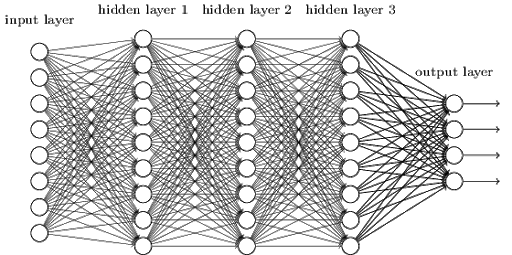
\includegraphics[scale=0.5]{fnn}
                \caption{A Feedforward Neural Network with 3 hidden layers(ref. Michael A. Nielsen, Neural Networks and Deep Learning, Determination Press', 2015)}
                \label{fig:fnn}
            \end{figure}
            This general but still basic form of Neural Network is known as \textit{Feed Forward Neural Network} Fig. \ref{fig:fnn}. 
        \section{Training}

            There are still a couple of important pieces left to define to develop a properly working Neural Network. For instance, how are parameters computed? And in particular, with respect to what we compute them? 
            \subsection{Loss Function}
                Before we realized that our goal is to maximize the approximation of the ground-truth input-output relation that lies under the data, therefore there is a need to
                introduce some metric to quantify this approximization. Call \textit{loss function} $ L(f_{\theta}\left(x\right), y) \colon \mathcal{Y} \times \mathcal{Y} \to \mathbb{R_+}$ 
                such metric. Common choices are (ref.):
                \begin{itemize}
                    \item Least Square: $\norm{f_{\theta}\left(x\right) - y}^2$ for regression tasks 
                    \item Binary Cross-Entropy: $y \log (f_{\theta}(x))+(1-y) \log (1-f_{\theta}(x))$ for binary classification  
                    \item Categorical Loss Function: $-\sum_{c=1}^{C} y_{c} \log \left(f_{\theta}(x)_c\right)$ for multicategory classification with $C$ classes.
                \end{itemize}
                Intuitively, a good loss function will map bad approximations to high values and good approximations to smaller ones.
                Nevertheless, those are only point-wise estimates of the error, hence the best empirical solution learnable from the training set $ S $ would be 
                \begin{equation}
                    \label{erm}
                    \displaystyle{  \min_{\theta}  \frac{1}{n} \sum_{i=1}^{n} L\left(f_{\theta}\left(x_{i}\right), y_{i}\right) }
                \end{equation}
                which is called \textit{empirical risk minimization}.
            \subsection{Gradient Descent}
               So far we have described, given an input $ x $, how we can compute the output of a feedforward neural network by means of compositions of dot products 
               and non-linear transformations between matrices, starting from the first to the very last of the layers in what is called a \textit{forward pass}. As it turns out, to attempt to solve \ref{erm} we need to follow the exact
               opposite path. Indeed, every optimization algorithm used in practice makes use of the same subroutine called Backpropagation (ref.  ) introduced in the 1970s, which allows to compute, starting from the output layer
               and going backwards, the partial derivative of the loss function with respect to each weight in the network. Moreover it does so efficiently requiring only one \textit{backward pass}.

               Let $i^l = W_l z_{l-1} + b_l$ be the weighted input to the $l$-th layer, then the key observation is that the only way $ W_l $ can affect the loss function is by affecting linearly
               the next layer which in turn affects its next layer and so on. In particular assume we add a little change $\Delta i_{j}^{l} $ to the $j$-th 
               element of $ i^l $ so that the neuron will output $ \sigma \left(i_{j}^{l} + \Delta i_{j}^{l}\right) $, this change will
               eventually propagates in the network causing the overall loss $LS$ to change by an amount $\frac{\partial LS}{\partial i_{j}^{l}} \Delta i_{j}^{l}$. For brevity,
               denote the gradient of the weighted input on the j-th neuron $ \delta^{l}_{j} = \frac{\partial LS}{\partial i^{l}_{j}} $, then the following holds:
               \begin{equation}
                 \delta^{L}_{j} = \frac{\partial LS}{\partial i^{L}_{j}} = \frac{\partial LS}{\partial z^{L}_{j}}\frac{\partial z^{L}_{j}}{\partial i^{L}_{j}} \\
                                =\frac{\partial LS}{\partial z^{L}_{j}} \sigma_{L}^{\prime}(i^{L}_{j})
               \end{equation}
               and equally, taking into account the whole output layer
               \begin{equation}
                    \label{bp1}
                    \delta^{L}=\nabla_{z^L} LS \odot \sigma^{\prime}(i^{L})
               \end{equation}
               where $ \odot $ is the element-wise product and $ \nabla_{x} $ the vector of the partial derivatives $ \partial LS / \partial x $. 
               That is, the gradient with respect to the weighted input to the last layer is given, using the chain rule, by the gradient with respect to the activation of the last layer times the derivative
               of the last activation function. Similarly, for any hidden layer $ l $ we note that:
               \begin{equation}
                \label{bp2}
                    \delta^{l}=\left((W^{l+1})^{T} \delta^{l+1}\right) \odot \sigma^{\prime}(i^{l})
                \end{equation}
                When we apply the transpose weight matrix, $(W^{l+1})^{T}$, think intuitively of this as moving the previous layer's gradient backward, giving a measure of the gradient at the output of the $l$-th layer. 
                We then take the product $\sigma^{\prime}(i^{l})$ which again moves the gradient backward through the activation function in layer $l$, giving the gradient of the weighted input to layer $l$.

                By combining \ref{bp1} with \ref{bp2} we can compute the gradient $\delta^{l}$ for any layer in the network. We start by using \ref{bp1} to compute on the last layer, 
                then apply equation \ref{bp2} to compute $\delta^{L-1}$, then the same equation again to compute $\delta^{L-2}$, and so forth, 
                all the way back until the input layer. Since our intent is to retrieve the gradients for every weights of the network, we are left to 
                show how $ \delta^l $ relates to them, here we provide such relation without giving an explicit proof which instead can be found in many
                texts like (ref Nielsen chapter 2).
                \begin{equation}
                    \frac{\partial LS}{\partial b^{l}_{j}} = \delta^{l}_{j}
                \end{equation}
                \begin{equation}
                    \frac{\partial LS}{\partial w^{l}_{i,j}} = z^{l-1}_i \delta^{l}_{j}.
                \end{equation}
                Remark how we already know how to compute each element on the right sides of these equations, moreover, given that the activation function
                and its derivative is efficiently computable, we will be able to efficiently get the seeked gradients in just one pass.
                It is worth mention that Backpropagation is actually a special case of a more generic set of programming techniques that go under
                the name of \textit{Automatic Differentiation} (Ref. ) to numerically evaluate the derivative of a function specified by a computer program.
                Such techniques are usually implemented in modern numerical libraries building variations of a data structure called \textit{computational graph}.
                Well known examples are \textit{Autograd} in \textit{Pytorch} (Ref. ) or \textit{GradientTape} in \textit{TensorFlow} (Ref. ).

               What does it mean to be able to compute partial derivatives of the loss? It means being able to understand where and how 
               the loss decreases and thus we can exploit such information to find better and better weights solutions. 
               This is the idea behind the Gradient Descent algorithm (Ref. ). In particular, the gradient of a weight is nothing but the
               direction inside the weight-space where the loss function is increasing, therefore what we want to do is to follow the opposite
               direction. Formally, this translates in the following weight update rules:
               \begin{equation}
                    w^{t}_{l} \rightarrow w_{l}^{t+1}=w^{t}_{l}-\frac{\eta}{n} \sum_{j} \frac{\partial LS_{x_{j}}}{\partial w^{t}_{l}}
               \end{equation}
               \begin{equation}
                b^{t}_{l} \rightarrow b^{t+1}_{l}=b^{t}_{l}-\frac{\eta}{n} \sum_{j} \frac{\partial LS_{x_{j}}}{\partial b^{t}_{l}}
               \end{equation}

            where $w_{l}^{t}$ are the values of the weights for layer $l$-th during the $t$-th pass, $\eta$ is a small positive constant called \textit{learning rate}
            chosen by the user accordingly and the gradients are averaged among all samples in the training set. 
            \begin{figure}[h!]
                \centering
                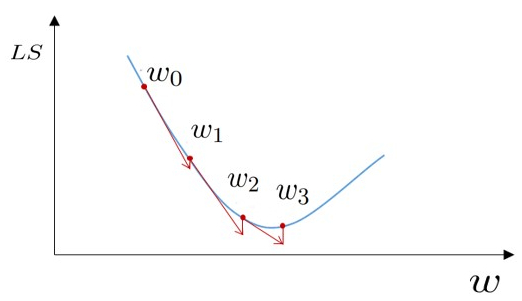
\includegraphics[scale=0.5]{gd}
                \caption{A 1-D representation of 4 gradient descent steps}
                \label{fig:gd}
            \end{figure}
            Most importantly, note how we take the negative of the gradients, meaning that we are following the direction in which the loss decreases Fig. \ref{fig:gd}. The distance
            between two consecutives weights $\Delta_{w^t}$ well be directly proportional to both the learning rate picked and the averaged gradient.

            In practice, however, very often we are deling with thousands or milions of data points, becomes unfeasable to compute every pass over
            the entire training set, thus what is done is to split the data into so called \textit{mini-batches} and then apply the
            update rules on each mini-batch until we scanned the whole data. The entire scan is called \textit{epoch} and the 
            resulting algorithm Stochastic Gradient Descent (Ref. ). Lastly, the size of a mini-batch is another hyperparameter 
            that should be tuned by the developer, keeping in mind that the bigger the size the more stable will be our training
            the smaller the size the faster the training.

            \begin{figure}[h]
                \centering
                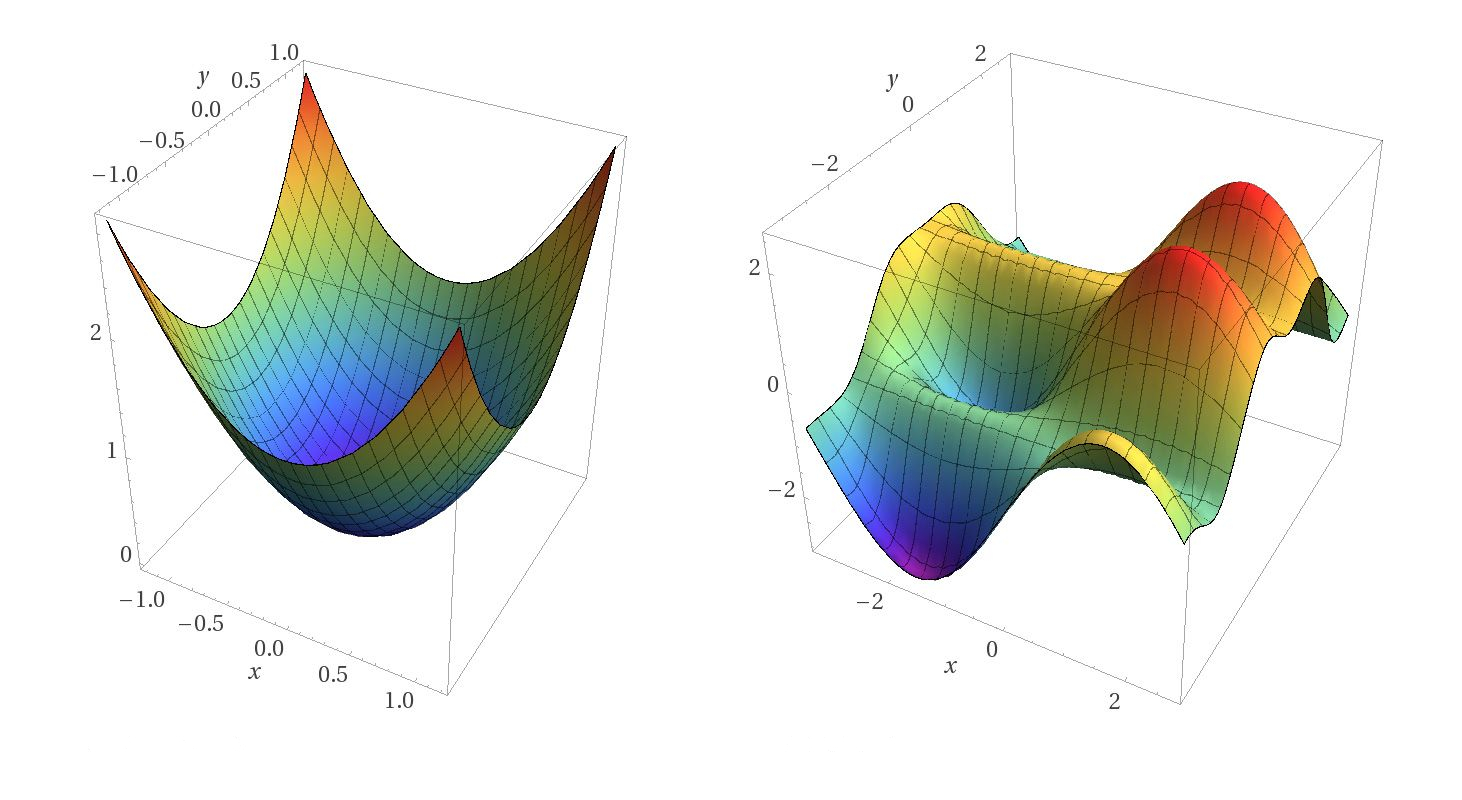
\includegraphics[scale=0.25]{conv_nonconv}
                \caption{Convex and Non-convex optimization landscapes}
                \label{fig:convnonconv}
            \end{figure}
            As stated earlier, neural networks can model extremely non-convex input-output functions therefore in principle there
            is no guarantee that Gradient Descent will find the optimal solution to \ref{erm} Fig. \ref{fig:convnonconv}.
            Indeed, the optimal solution would be the global minimum of our weighted loss function but there is no apparent
            way for the algorithm to distinguish between global, local minimum or saddle points Fig. \ref{fig:globlocsad}.
            However, it turns out that in practice Gradient Descent works fairly well once we correctly tune
            hyperparameters and run the algorithm from different initial values. (Ref .)
            Moreoever, lately authors have been proposed different methods to improve the convergence and the efficiency by 
            smart changes of the learning rate during the training process (ref . cyclical learning rates) 
            \begin{figure}[h]
                \centering
                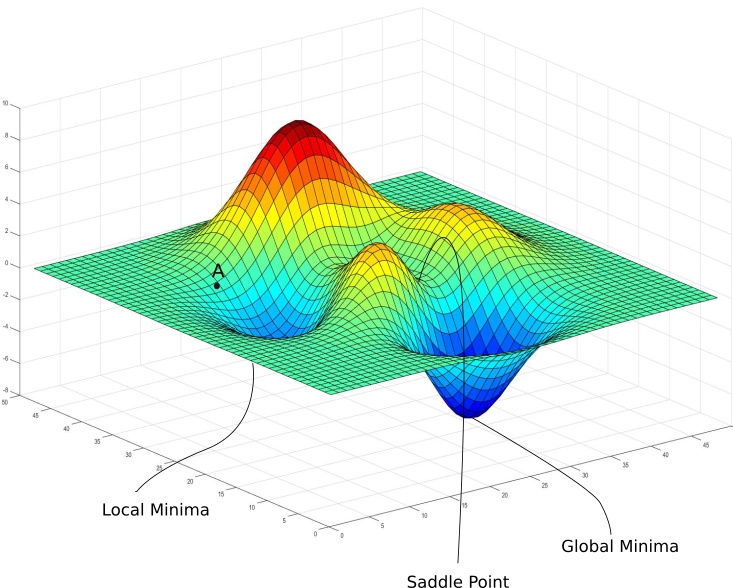
\includegraphics[scale=0.35]{globlocsad}
                \caption{Visualization of global, local and saddle points. How can A reach the global minimum?}
                \label{fig:globlocsad}
            \end{figure}

        \section{Activation Functions}
            
            We have seen how the learning process works optimizing the empirical risk by means of gradients computation.
            Therefore to be able to optimize anything, a neural network needs to have only differentiable components.
            However, before in \ref{step} we discussed the so called \textit{step function}, an activation function that, 
            even if biologically inspired and easier to justify, is not differentiable at the origin and the derivative is 0 elsewhere.
            Thus if we think again about how Backpropagation works, we see that employing such activation function would make the weight updates impossible
            since already $ \delta^{L} $ would be either undefined or 0.

            To deal with this issue, one of the first proposed activation functions was an approximation of the step function known as \textit{sigmoid} (Ref. ) 
            \begin{equation}
                \textnormal{sigmoid}(x) = \frac{1}{1 + e^{-x}}
            \end{equation}
            which is differentiable everywhere with continuous derivatives (property that we will refer as \textit{smoothness} through the chapters) and
            maps to $ [0, 1] $ values.
            \begin{figure}[h]
                \centering
                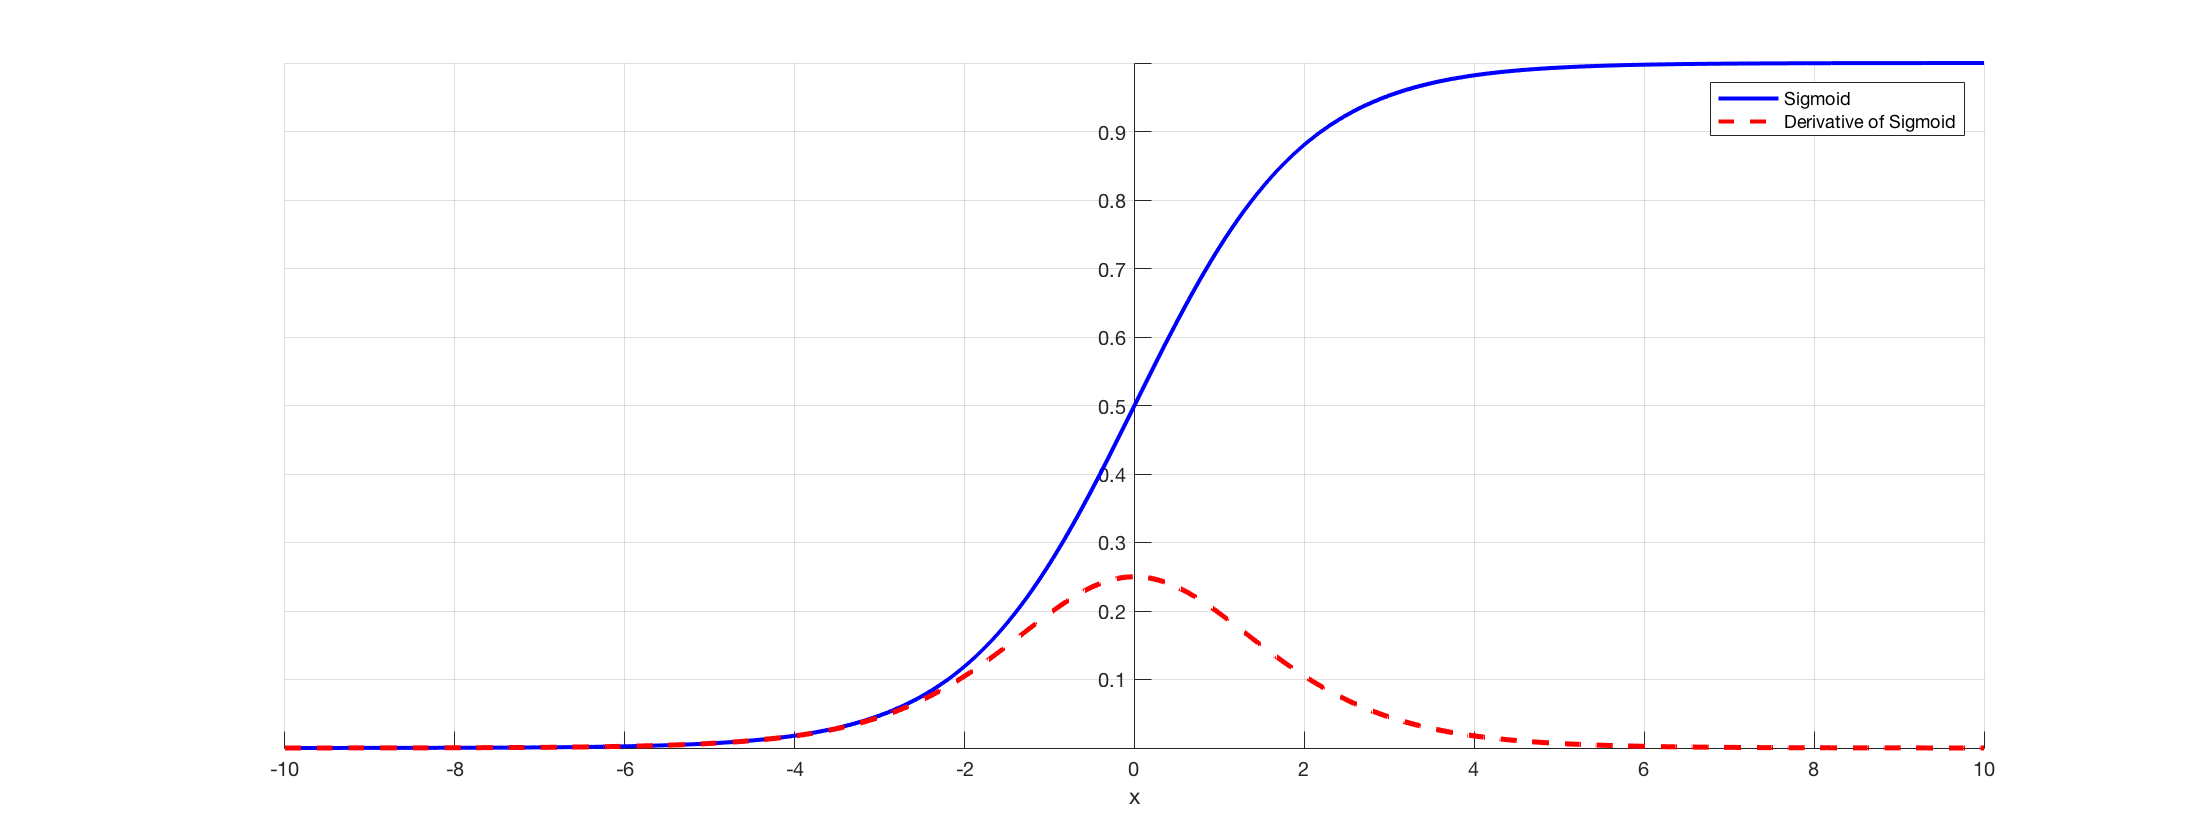
\includegraphics[width=1\textwidth]{sig_der}
                \caption{Plot of the Sigmoid function and its first derivative.}
                \label{fig:sigmoid}
            \end{figure}
            Nevertheless, as the number of layers increases and the network becomes sufficiently deep, the sigmoid suffers from the \textit{vanishing gradient} problem (Ref. ) Fig. \ref{fig:sigmoid}
            due to its derivative being $[0, 0.25]$ bounded. Mainly for this reason it is not widely adopted in practice.

            More in general, the sigmoid lies inside a class of activation functions known as \textit{squashing} i.e. monotonically non-decreasing functions $\varSigma$
            that satisfy
            \begin{equation}
                \lim_{x \to - \infty} \sigma(x) = c, \quad 
                \lim_{x \to \infty} \sigma(x) = 1.
            \end{equation}
            For example, another kind of activation function of this type is the \textit{hyperbolic tangent}, defined as
            \begin{equation}
                \tanh (x)=\frac{\exp \{x\}-\exp \{-x\}}{\exp \{x\}+\exp \{-x\}},
            \end{equation}
            which was find to allow for universal expressivness of nets (Ref. ). However, as for the sigmoid, squashing functions tend to be prone to vanishing 
            and exploding gradients (Ref. ).

            Nowadays, the most used activation function in neural networks for different applications is the \textit{rectifier linear unit} (ReLU),
            first introduced in (Ref. Hahnloser et al. in 2000) and defined as the positive part of its argument
            \begin{equation}
                \textnormal{ReLU}(x) = \max(0, x),
            \end{equation}
            allows for efficient training and alleviates the exploding gradient problem (having derivative either 0 or 1), introducing only one point of
            non-differentiability. Moreover, it promotes \textit{sparsness} in the network, which is usually beneficial (Ref. ). One problem with ReLUs though 
            is that the neuron's value, that get pushed to a big negative number, might stay stucked in 0 for essentially all inputs, in a so called \textit{dead state}.
            If many neurons in the network die this can afflict the model capacity and can be seen as a form of vanishing gradient problem. To overcome this problem,
            a slighlty different activation functions can be used, called \textit{leaky ReLU} (Ref. ):
            \begin{equation}
                \operatorname{Leaky ReLU}(x)=\left\{\begin{array}{ll}
                    x & \text { if } x \geq 0 \\
                    \alpha x & \text { otherwise },
                    \end{array}\right.
            \end{equation}
            where $\alpha > 0$ is a user-defined constant usually set to small values such as 0.01. Even if this solutions solves the dying neurons problem, it does
            affect the sparseness property of ReLUs.
            
            By definition, the mean of ouput values from a ReLU is always positive. \textit{Exponential linear unit} (ELU) try to normalize their inputs:
            \begin{equation}
                \label{elu}
                \operatorname{ELU}(x)\left\{\begin{array}{ll}
                    x & \text { if } x \geq 0 \\
                    \alpha(\exp \{x\}-1) & \text { otherwise },
                    \end{array}\right.
            \end{equation}
            saturating negative values at a user-defined value $- \alpha$ which is usually set to 1. Conversly to ReLU and LeakyReLUs, the derivative is continuous
            therefore the function is smooth and for the negative values is defined as $ELU(x) + \alpha$.

            Finally, one more recent activation function which gained a lot of attention is the \textit{Swish} function (Ref. ):
            \begin{equation}
                \operatorname{swish}(x)= \operatorname{sigmoid}(x) * x,
            \end{equation}
            
            \begin{figure}[hb!]
                \centering
                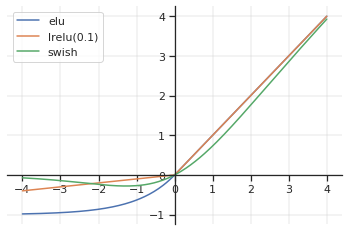
\includegraphics[scale=0.50]{afunctions}
                \caption{ELU, LeakyReLU($\alpha=0.1$) and Swish functions plotted together. It can be seen that they mostly differ for negative values whereas behaving very similar to ReLU for positive arguments.}
                \label{fig:afuncs}
            \end{figure}
            which again does look like another approximation of a ReLU Fig. \ref{fig:afuncs}, but in this case it manages in not loosing any useful property. Indeed, since
            it also saturates at 0 for negative values, it allows for sparsity and being smooth around 0 it helps reducing dying neurons. Lastly, around 0 negative 
            values are kind of preserved which may still be relevant to patterns in the underlying data.
            Swish function proved to consistently match if not outperform ReLU networks in different domains (Ref. ), and more recent studies showed how this function
            can also help in training more \textit{robust} networks (Ref. Smooth Adversarial training).

            Along with this list of more 'traditional' activation functions, which we will call \textit{fixed} activation functions, there is a whole branch of
            more sophisticated solutions, where the idea is to \textit{learn} the function's optimal shape employing suitable parametric functions. 
            Such functions can then be trained together with other weights of the net using backpropagation and gradient descent. Moreover, following the terminology
            introduced in (Ref Scardapane t al KafNets) we can again distinguish between two classes of this learnable activation functions: the so called
            \textit{parametric activation functions} and \textit{Non-parametric activation functions}. The former being usually a parametrization of a fixed 
            activation function involving few constant parameters, whereas the latter is called non-parametric due to the number of parameters that can in principle
            grow without a bound and involves more complex shapes. At the end of this chapter we introduce a recently proposed class of non-parameteric activation functions,
            called \textit{Kernel-Based Activation Functions} which will then be the main tool used in the following chapters to try to build more robust neural networks.    


        \section{CNNs: Convolutional Neural Networks}

            In computer vision, in particular for image processing tasks, we can make the assumption that the input to the model will be an image. 
            How well do feedforward neural networks adapt to such inputs? It turns out that we need to introduce several changes in the architecture in order to expect 
            them to work properly. Take for example the famous dataset \textit{ImageNet} which consists of more than $ 14 $ milions of images,
            all of which made of $ 256 \times 256 \times 3 $ pixels. Every fully connected neuron in the first layer would have $ 256 * 256 * 3 =  196608 $ weights,
            thus for a neural network with $ 1000 $ of such neurons, which is a very small number of units in practice, we would already need to train almost $ 200 $ milions of parameters,
            which requires a lot of resources. Therefore feedforward neural networks do not scale well to bigger images. More importantly, assume our task is to 
            classify an image, from the point of view of such models, if we take an image $x$ and perform a translation to, lets say, the right for few pixels, with high 
            probability it will look like a completly different image from the point of view of the net and will probably be classified differently, even if 
            from our point of view is clearly the same image. In some sense, there is no apparent way in which fully connected neural networks can take advantage of 
            concepts such as \textit{locality} or \textit{translation invariance} that are intrinsic to images.
            
            To circumvent these limitations, reasearchers have developed a specific architecture targeted for computer vision tasks called \textit{Convolutional Neural Network} (CNN) (Ref. ).
            In a standard CNN, every layer is $3$-dimensional $(Width \times Height \times Dept) $ to reflect the fact that we are always dealing with images 
            and each neuron is connected only to a constant number of nearby neurons in the previous layer, shrinking down the number of total weights required.
            Layers can be either \textit{convolutive layers} or \textit{pooling layers} or \textit{fully-connected layers}, the latter being a normal hidden layer.

            A convolutive layer takes in input $W \times H \times C_{in}$ neurons from the previous layer and outputs $W \times H \times C_{out}$ neurons, where $ C_{out}$
            is the number of filters used by the layer. A filter $F$ is a $K \times K \times C_{in}$ matrix of trainable weights, with $K>0$ typically a small integer, which is used to
            compute a 2-dimensional activation map by sliding (convolving) across the width and height of the input. At each slice of input 
            $ \mathbf{x_{ij}} = (x^{1}_{ij}, x^{2}_{ij}, \ldots, x^{C_{in}}_{ij})$ that it touches, it computes the dot product $ F^{T}X_{ij}$
            where $X_{ij}$ is the $K \times K \times C_{in}$ window centered at $\mathbf{x_{ij}}$.
            \begin{figure}[hb!]
                \centering
                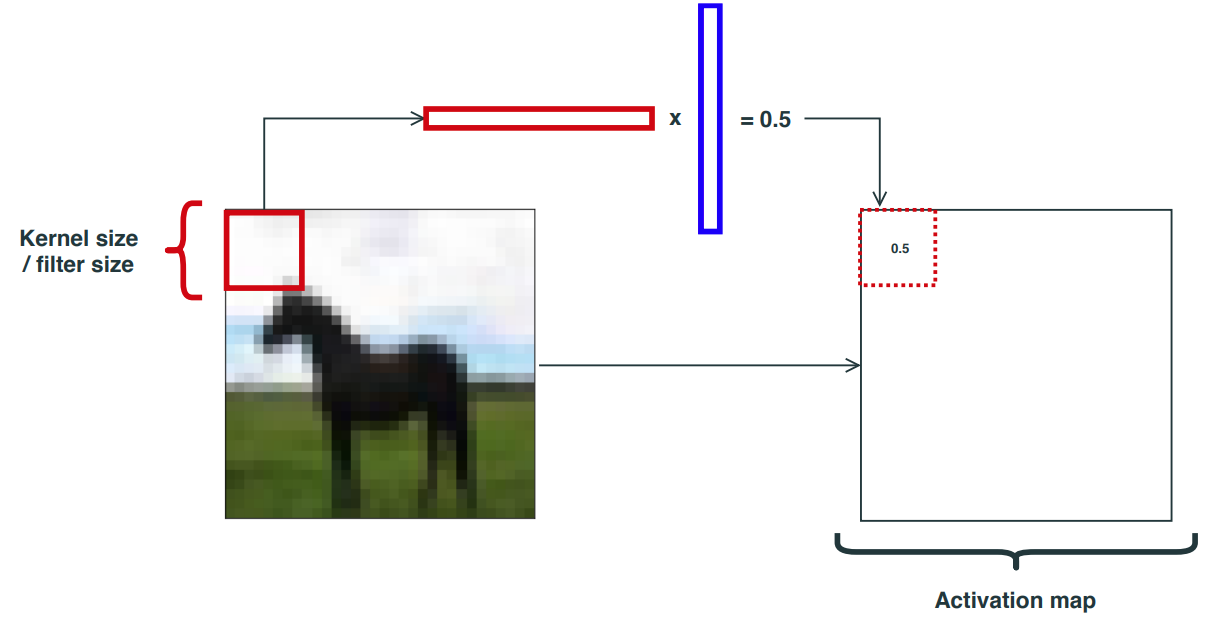
\includegraphics[scale=0.30]{convolution}
                \caption{A convolution that produces the first element of the activation map for the given filter.}
                \label{fig:conv}
            \end{figure}
            Intuitively, through backpropagation we learn filters tha are capable of recognizing specific shapes in the image, which we can see as features,
            starting from very concise ones in the early layers to more global ones towards the end layers as the receptive field gets larger(Ref. ). 
            Typically, as for normal neural networks, we apply a non-linear transformation after each convolutive layer and by stacking many of these Convolutional
            layers we get a convolutional network.
            
            \begin{figure}[b!]
                \centering
                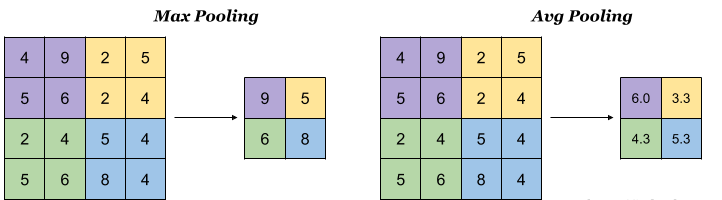
\includegraphics[scale=0.30]{pooling}
                \caption{Max (left) and Average (right) pooling layer with 2x2 window size.}
                \label{fig:pooling}
            \end{figure}
            Going deeper in the network, as we learn global features, it might be convenient to reduce the width and the height dimensions. For this reason CNNs employ pooling layers
            that filters the inputs by some aggregation metric, such as average or max values. Similarly to a convolution, we specify a 
            $ K \times K $ window on which we apply the chosen metric. For example, let $z^{l-1}$ be a $(64,64,12)$ dimensional
            input to a max pooling layer with window size $2\times2$, then, sliding again across width and height of $z^{l-1}$, we take the max value for each
            $ 2 \times 2 $ input patch that we touch. The output will then be a $ (32, 32, 12) $ dimensional vector of max valued neurons Fig. \ref{fig:pooling}. 


            The complete architecture of a textbook CNN is a composition of 2 subarchitectures:
            \begin{itemize}
                \item A sequence of interleaved convolutive and max-pooling layers
                \item A \textit{flatten} layer to reduce the last convolution to a 1-dimensional vector, followed by a sequence of fully connected layers to obtain the final score vector.
            \end{itemize} 
            put together resulting in a  \textit{two-staged architecture}: 
            \begin{figure}[h!!]
                \centering
                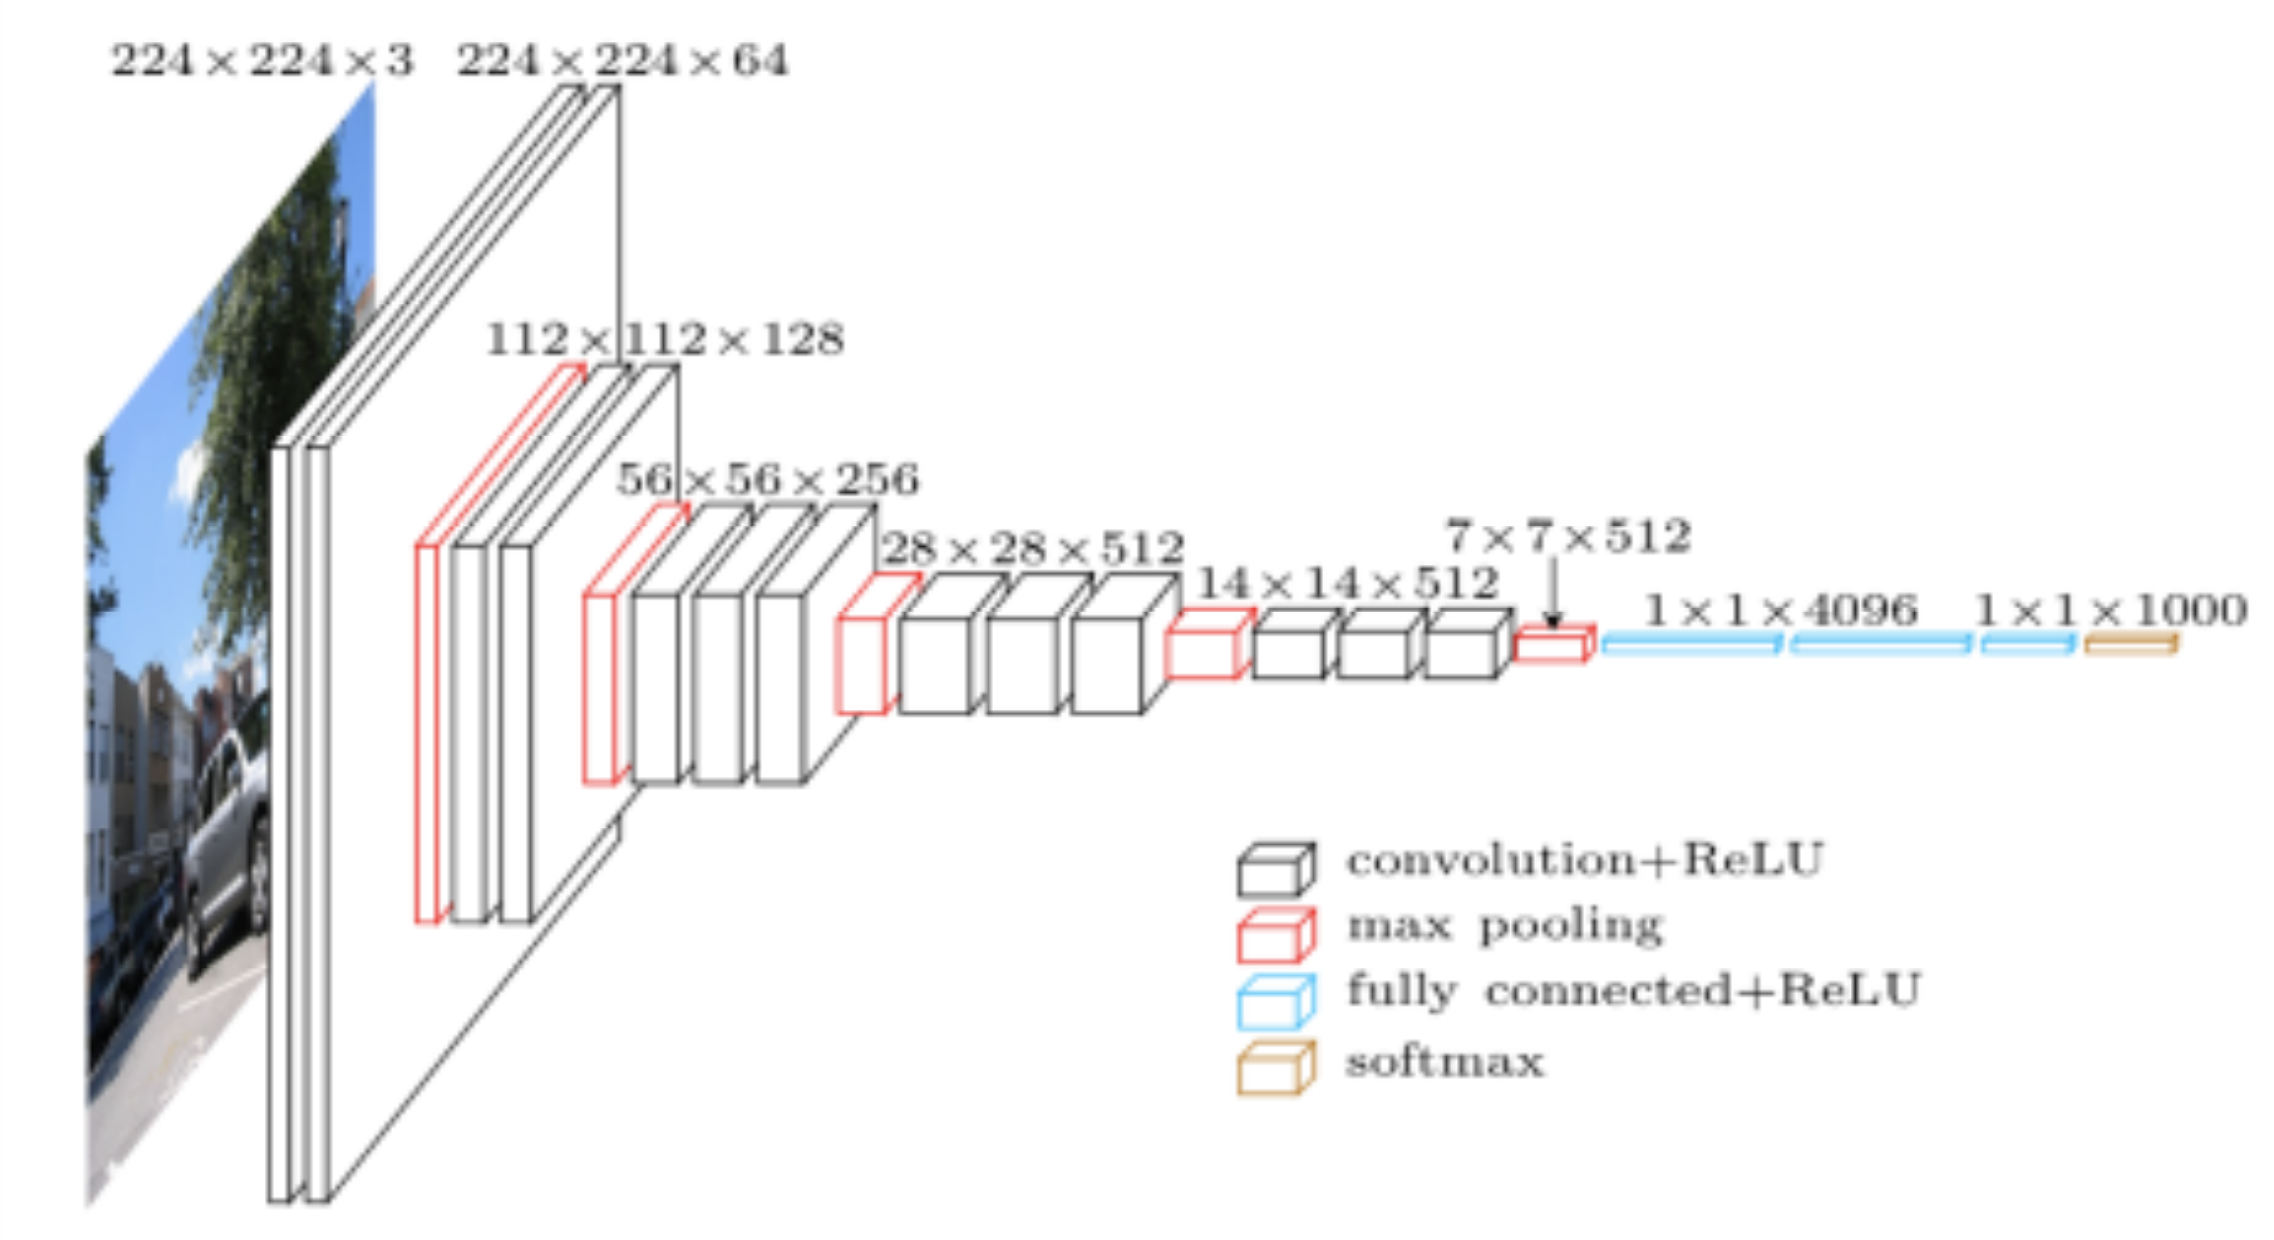
\includegraphics[scale=0.11]{cnnarch}
                \caption{General Architecture of CNN for ImageNet (Ref. ).}
                \label{fig:cnnarch}
            \end{figure}
            
            Even if we can already reach good accuracies with such a basic architecture, modern CNNs employ many smart variations to improve even more the performance,
            as we shall see in the next section. 

        \section{From Neural Networks to Deep Neural Networks}
        Assume to develop a CNN as we have just seen to perform an image classification task. If the built network is sufficiently large, and the chosen dataset limited
        in number of samples, it might happen that our network will \textit{memorize} the entire trainset instead of learning anything useful from it (Ref. 
        UNderstanding DL requieres rethinking generalization). The described scenario is an infamous problem in learning theory and goes under the name of \textit{overfitting},
        i.e., instead of trying to learn the ground-truth distribution underlying the data, our model somehow tries to interpolate the training set, 
        resulting in poor generalization capabilities. 
        Early techniques to takle overfitting involve detection methods such as \textit{early stopping} (Ref. On Early Stopping in Gradient Descent Learning) 
        or basic prevention methods such as \textit{regularization} (Ref. Regularization Theory and Neural Networks Architectures),
        where we try to penalize learning big-valued weights, which are syntoms of overfitting, by carefully adding penalization terms inside the optimization function.

        Despite the fact that the presented techniques are very effective in practice and can help mitigating the problem, they are usally not enough for high perfomances.
        Another form of regularization can be induced performing \textit{data augmentation} (Ref. AlexNet paper) which consists in virtually increasing the size of the train set applying
        , for each example in a mini-batch, one or more randomly sampled image transformation such as flipping, cropping, ecc. and then train on the resulting augmented
        trainset. Another idea to make the robust against slighlty perturbations hence more likely to generalize well is \textit{Dropout} (Ref. Alexnet paper).
        Droput extends the idea of data augmentation to the network itself perturbing the hidden layers instead of the inputs by randomly dropping some of the
        neurons. More formally, assume $z^l$ be the output of a generic layer $l$, then applying Dropout to the ouput means replacing $z^l$ during
        training with:
        \begin{equation}
            \hat{z^l} = z^l \odot m,
        \end{equation}
        where $m$ is a binary vector with entries taken from a Bernoulli distribution with probability $p$. It is important that Dropout gets applied only
        during training whereas at inference time the output of the layer is replaced with its \textit{expected} training value:
        \begin{equation}
            \mathbb{E}[\hat{z^l}] = p \cdot z^l. 
        \end{equation}
        Both data augmentation and Dropout were key components of \textit{AlexNet}, the first CNN to win an image classification
        contest by a big margin (Ref. AlexNet p).

        In 2014, the Oxford's Visual Group realized that they were able to reach better performances than AlexNet by stacking \textit{blocks} of layers instead of many 
        single layers one after the other. In particular, they proposed a block made of multiple convolution layers with $ 3 \times 3 $ kernel size and same 
        number of filters, followed by a $ 2 \times 2 $ max-pooling, periodically doubling the number of filters for deeper blocks (Ref. VGG). The resulting 
        architecture, known as in literature as \textit{VGG}, was however considerably demanding in terms of resources and this drove researchers to look 
        for solutions that matched the performances whereas decreasing the number of weights. Such goal was achived soon after with \textit{GoogleNet}
        which made use of two novel modules inside the network: the \textit{inception block} and the \textit{global average pooling} (Ref. GoogleNet). The former 
        being the first attempt at process in parallel the same input with different levels of granularity, somehow allowing to embed multiple layers within a single
        one Fig. \ref{fig:inception}
        \begin{figure}[h!]
            \centering
            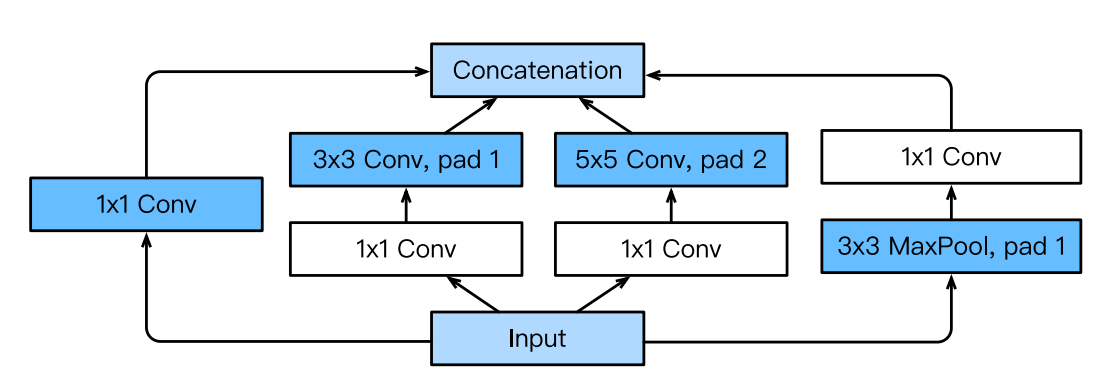
\includegraphics[scale=0.25]{inception}
            \caption{Inception Block overview, $1\times 1$ convolutions are used to reduce the number of filters lowering complexity. Source: Dive into Deep Learning, chapt. 7.4}
            \label{fig:inception}
        \end{figure}
        , and the latter used as a substitute for the flatten layer by taking the average value in each channel and then vectorizing them into a 1-dimensional vector. 
        This last step drastically reduces the number of weights needed in the second stage of the CNN. 
        
        Less than one year later, another breakthrough technique was developed: the \textit{Batch Normalization} (BN), a simple heuristic that 
        allowed to train deep neural nets significantly better  (Ref. ). BN works by normalizing and learning to scale the mean and the variance of a layer's output
        in the following way: consider $i_1, i_2, \ldots, i_B$ to be the values of a generic given neuron during a mini-batch. Then with Batch Normalization,
        we first normalize them by:
        \begin{equation}
            i_j = \frac{i_j - \mu}{\sqrt{\sigma^2 + \epsilon}},
        \end{equation}
        with $\mu$ and $\sigma$ being respectively the mean and the variance of the mini-batch values. Then,
        we rescale them by:
        \begin{equation}
            i_j = \alpha i_j + \beta,
        \end{equation}
        where $\alpha$ and $\beta$ are trainable parameters computed with respect to every neuron in the layer.
        Nowadays, it is believed that the reason behind the effectiveness of BN is likely due to its effect on the 
        optimization landscape (Ref. ), which gets smoothed, hence the speed-up in convergence and better
        generalization properties.

        Having developed tools that bypass exploding and vanishing gradients, that allow for faster convergence
        and better generalization, one may be tempted in see what happens when we keep stacking more and more layers.
        After all, the intuition we gained from the general trend in CNNs is that the deeper the network, the better
        the learning. However, this belief was not matched by experiments. Indeed, for very deep 
        straightforward neural networks, we are likely to experiment a \textit{degradation}(Ref. ref made by resnetpaper) of accuracy perfomances
        which is not caused by overfitting i.e. it leads both to higher test and training error Fig. \ref{fig:degradation}.
        \begin{figure}[h]
            \centering
            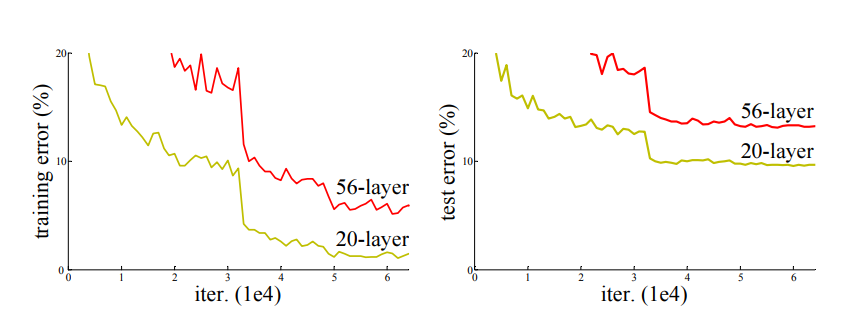
\includegraphics[scale=0.35]{degradation}
            \caption{Source: Deep Residual Learning for Image Recognition}
            \label{fig:degradation}
        \end{figure}
        To approach the problem we can start with the following remark: if we assume a shallow
        network $ \mathcal{F} (x) $ for a given task reaches an accuracy $a$, then by adding identity layers on such network i.e. layers implementing the identity function,
        will result in a deeper network with again accuracy $a$, it can't get much worse.
        Building upon this argument, authors in (Ref. ResNet paper) showed that a deep network will rather
        learn a better mapping starting from $ \mathcal{F} (x) + x $ than from $ \mathcal{F} (x) $. 
        For this reason, they introduce the idea of \textit{skipping connections} or \textit{residual connections} where, 
        as the name suggests, we link the input of an earlier layer to the output of a deeper layer, skipping
        over the layers in between Fig. \ref{fig:residual}.
        \begin{figure}[h]
            \centering
            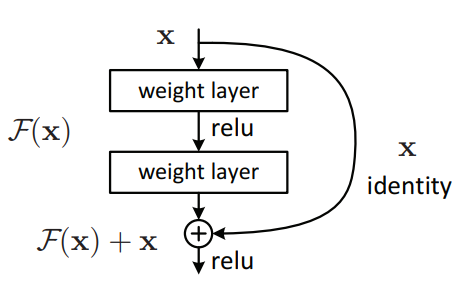
\includegraphics[scale=0.35]{residual}
            \caption{Source: Deep Residual Learning for Image Recognition}
            \label{fig:residual}
        \end{figure} 
        If $x$ has different dimensionality, we can rescale it using a $ 1 \times 1 $ convolution. A neural network 
        that makes use of many residual connections is called \textit{ResNet} Fig. \ref{fig:resnet}. 
        \begin{figure}[h]
            \centering
            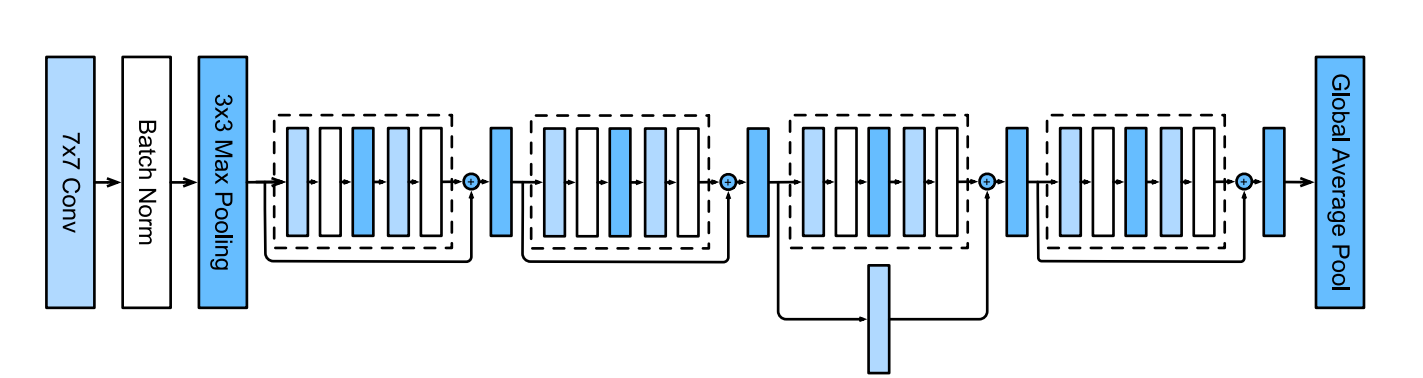
\includegraphics[scale=0.30]{resnet}
            \caption{Source: Dive Deep into Deep Learning}
            \label{fig:resnet}
        \end{figure}

        Thanks to the methodologies introduced so far, we are capable of building non-degenerative CNNs that scale up to hundreds of layers
        and are currently state-of-the-art in many domains.


    \chapter{Adversarial Examples Theory}

    In recent years, AI-based systems are finding an ever growing number of applications in the industry, ranging from medical, multimedia, telecomunications, to even military, political and legal sectors. 
    As a consequence of the importance of such systems to the modern world, it is currently reasonable to think that they might become potential threats to the eyes of
    malicious agents such as hackers, business rivals as well as governments, which may seek to circumvent them. For simplicity, we name any of these malicious entity: \textit{adversary}. 
    Inside academia, there is a vast literature on the topic and many attacks and defenses have been devised by researchers towards different types of intelligient systems for both supervised (Ref. Intriguing Properties)
    and unsupervised models (Ref. s data clustering in adversarial settings secure?) with no exception for Neural Networks. Even better, since, as we have seen, DNNs reach best performances among ML systems 
    in many applications, recent research efforts are especially directed in assessing the \textit{robustness} of DNNs. In this thesis we will stick to the same trend.

    In the context of classification, one of the many distintions that we can make about types of attacks is wether the objective of the attack is to just fool the classifier making it mislabel 
    a given sample $ x $, or targetting the classification towards a specific class $ \hat{y} $ where, given a sample-label pair $ (x, y) $ with $ \hat{y} \neq  y $, our classifier will be tricked in
    believing that the correct classification is indeed $ \hat{y} $. We name this two different scenarios \textit{indiscriminate} and \textit{targeted} attacks respectively. Moreover, despite the fact that the attack is targeted 
    or not, we define three inherently different attacks types against a classifier:
    \begin{itemize}
        \item \textit{Data Poisoning:}
        here the adversarial introduces \textit{poisoned examples} into the data. Poisoned examples can either be mislabeled examples, with the examples correctly belonging to the domain space described
        by the data, or they can be anomalies for the domain. For instance, if data describes birds, a ship should be considered very odd and thus poisoned (Ref. ).
        \item \textit{Reverse Engineering:}
        usually crafted against rule-based classifiers, such attack consists in querying the model to retrieve sensible information about its decision rule or the data on which it was trained (Ref. ).
        \item \textit{Test Time Evasion:}
        as the name suggests, here the attack is performed at test time by a careful \textit{perturbation} of the the sample in a way that the transformation is neither human percetible nor
        easily detected by the system, but as powerfull that the classifier's decision now disagrees with a human consensus (Ref. Explaining and harnessing adversarial examples).
    \end{itemize}
    As shown for the first time in (Ref. Intriguing Properties of..), DNNs are drastically prone to Test Time Evasion attacks and, more importantly, unaware networks can easily be fooled in a matter of
    few lines of code by anyone who knows the basics of any modern deep learning framework. For this reason, we will dedicate this section to a formal introduction of the problem, and the rest of 
    the thesis in the development of a new approach that aims to improve the resiliency - in jargon, \textit{Robustness} - of Neural Networks against today's Test Time Evasion attacks. 

    \section{Another Optimization problem}
        
        To get a Test Time Evasion attack working, any adversary needs to know the true class of the input he is manipulating. Indeed, the perturbation needs to be done in such a way that 
        the resulting perturbed input will cross the true class decision region, in the output space of the model, to move to another decision region (which is specific to the targeted category in case of a targeted attack).
        However, due to an high number of weights and non-linearities involved in a forward pass, we usually don't know how DNNs actually make their predictions, instead we delegate the job of learning 
        how to make decisions to Gradient Descent during training. Therefore, how does an adversary learn how to craft such untangible yet precise perturbations? Well, he relies again on Gradient Descent, more precisely,
        on back propagation. Recall that, in the previous section, we learned how to compute the gradient $\frac{\partial LS}{\partial w^{l}_{i,j}}$ with respect to any weight $ w^{l}_{i,j} $ of the 
        network, nevertheless, nothing prevents us to push even further automatic differentiation and compute the gradient of the loss with respect to the input $x$ with just as much effort. 
        This quantity will tell us how small changes to the image itself affect the loss function.
        
        Since the goal of the adversary is to make the classifier mislabelling the input, and since we can optimize a function with respect to the input, we can devise an indiscriminate attack by just
        solving the following optimization problem:
        \begin{equation}
            \displaystyle{\max_{\hat{x}} \operatorname{LS}\left(f_{\theta}\left( \hat{x} \right), y\right)},
        \end{equation}
        where $\hat{x}$ is called \textit{adversarial example} and is nothing else that an approximation of the original input $x$. However we also need to characterize the fact that $\hat{x}$ must be very
        close to $x$. In fact, with this settings we could simply transform completly the input to make it equal to another input $x^{\prime}$ which belongs to a different class and would still be
        a valid solution. But this is clearly in contrast with the principle of being an human imperceptible perturbation! Thus denote $\delta \in \mathcal{X}$ to be the perturbation applied
        to the input $\hat{x} = x + \delta $, then the adversary will actually want to solve:
        \begin{equation}
            \label{attackobj}
            \displaystyle{\max_{\delta \in \Delta} \operatorname{LS}\left(f_{\theta}\left( x + \delta \right), y\right)},
        \end{equation} 
        where $\Delta$ denotes the set of any admissible small perturbation. Again, this is something we cannot implement straightaway since it is not clear from a mathematical perspective how to
        explicitly construct the set of all valid small perturbations, even if this is what the adversary is ideally trying to achieve. In practice, what is done is to stick to some mathematical metric such as 
        a specific norm for real vector spaces. For example, an effective metric which allows to fool many NNs, even with super small perturbations is the $L_{\infty}$ norm. The $L_{\infty}$ norm
        for a generic vector $z \in \mathbb{R^d}$ is defined to be:
        \begin{equation}
            \label{linfnorm}
            \|z\|_{\infty}=\max _{i}\left|z_{i}\right|.
        \end{equation}    
        Thus the space of allowed perturbations becomes:
        \begin{equation}
            \Delta = \{ \delta: \|\delta\|_{\infty} \leq \epsilon\},
        \end{equation}
        where $\epsilon$ is the size of the biggest perturbation allowed, i.e. if for example we are dealing with images, any pixel will be $[- \epsilon, \epsilon] $ perturbed and if $\epsilon$
        is chosen sufficiently small, the resulting image will be visually indistinguishable to the original one. However, other norms such as $L_2$ are also very common.

        How do we perform targeted attacks within this framework? Intuitively, the adversary will want to minimize the loss with respect to the targeted class but at the same time, he also wants 
        to be sure that the network will give the smallest confidence to the correct class. This translates into:
        \begin{equation}
            \label{targetedattack}
            \displaystyle{\max_{\delta, \|\delta\|_{\infty} \leq \epsilon }  (\operatorname{LS}(f_{\theta}(x + \delta), y) - \operatorname{LS}(f_{\theta}(x + \delta), y_{target}) )  }.
        \end{equation} 

    \subsection{Fast Gradient Sign Method}

        For the sake of discussion, we will now see how to actually solve the proposed maximization problems, restricting ourself to indiscriminate attacks, since the same solutions will also
        work painlessy for the case of targeted attacks. 

        In general, the basic idea behind every adversarial attack is to use Gradient Descent to maximize our objective until we converge towards a satisfying solution $\delta^{*}$,
        just as we did when we were training the network. Furthermore, in this case, we also have to take into account the bounds on the perturbation, which can be implemented by a projection  
        to the $[-\epsilon, \epsilon]$ norm-bounded space. In order to maximize loss, we want to adjust delta in the direction of this gradient, i.e., take a step:
        \begin{equation}
            \label{pgd}
            \delta^{t+1} = \delta^t + \alpha \cdot \nabla_{\delta^t} \operatorname{LS}\left(f_{\theta}(x+\delta^t), y\right),
        \end{equation}
        for some step size $\alpha$. Then, we clip $\delta^{t+1}$ to ensure the norm constraints, so in the case of $L_{\infty}$-norm:
        \begin{equation}
            \delta^{t+1} = \operatorname{clip} (L_{\infty}, \delta^{t+1}, [-\epsilon, \epsilon]),
        \end{equation}
        where clipping acts by projecting $\delta^{t+1}$ back to the $\epsilon$-bounded $L_{\infty}$ ball it moved outside.

        Now, if we want to climb the slope of the loss as much as possible we will want to take a very large step size. However, by doing so, we are probably going to stick out the $L_{\infty}$ ball
        and thus our delta will be either be projected to $\epsilon$ or $- \epsilon$ with high probability. Based on this principle, one of the first proposed attack simply considered the following update rule 
        for delta:
        \begin{equation}
            \delta = \epsilon \cdot sign(\nabla_{x} \operatorname{LS}\left(f_{\theta}(x), y\right)),
        \end{equation}
        and is known as the \textit{Fast Gradient Sign Method}(FGSM) (Ref. ). FGSM is a single step attack and works on the assumption that, in a very close neighbourhood of $x$, a DNN can be approximated with the 
        behaviour of a linear model. Consider a simple linear model $ g(x)  = W^Tx $, then $g(x + \delta) = W^Tx + W^T\delta $ and thus, if we want to maximize the effect of the perturbation 
        $ |g(x) - g(x + \delta) | $ under $\|\delta\|_{\infty} \leq \epsilon$ we better define $\delta = \epsilon \cdot sign (W^T)$. Even if the per-component shift is small, the overall shift 
        can increase way more if $x$ is high dimensional.
        
    \subsection{Projected Gradient Descent}
    
        The idea that the effect of any perturbation inside the $\|\delta\|\infty \leq \epsilon$ ball can be approximated, if not upperbounded, by taking the perturbation at the boundary which
        is given by the direction where the loss is most increasing might be a little too strong as an assumption. Indeed, as previously seen, the optimization landscape is often extremely
        non-linear, even for very small neighbourhoods, thus, if we want a stronger attacks, we likely want to consider better methods at maximizing the loss function than a single projected gradient step.

        A more effective and natural approach comes from iterating \ref{pgd} many times with small step sizes and projecting back whenever needed. The general algorithm is called \textit{Projected Gradient
        Descent} (PGD)(Ref. ):


            \begin{algorithmic}[0]
            \Procedure{PGD}{$\alpha, \epsilon$}
            \State $\delta \gets 0$
            \For{$i\gets 1, n$}
            \State $\delta \gets \delta + \alpha \cdot \nabla_{\delta} \operatorname{LS}\left(f_{\theta}(x+\delta), y\right)$
            \State $\delta \gets \mathcal{P}(\delta) $
            \EndFor
            \State \textbf{return} $\delta$
            \EndProcedure
            \end{algorithmic}
        Where $\mathcal{P}$ denotes the projection for the specific metric used. Nowadays, PGD, or slighlty variations of it are standard methods when 
        it comes to evaluate the robustness of a network.

        As for Gradient Descent, PGD is still limited by the possibility of getting stuck inside local maximum of our objective \ref{attackobj}.
        Mitigations of the problem might arise adding random restarts, i.e., running PGD multiple times from randomly picked starting deltas (within our norm restricted ball).
        It is infact important to note that it is likely that there are local optima which will be found if we start with $\delta = 0$ and that could be avoided with randomization. 
        Conversly, running multiple PGDs increases the runtime by a factor proportional to the number of restarts and it might not be practical in real world scenarios, especially when it is used
        as a subroutine to train robust models (Ref. Free Adversarial Training).

    \subsection{White, Grey and Black Box Attacks}

        In the aforementioned attacks, various implicit assumptions are made about the knowledge of the adversary. Biggio et al. in (Ref. Security evaluation of pattern classifiers under attack)
        , in alignment with the wider field of modern Cryptography, have advised making such assumptions explicit also for publications concerning the security of ML models. In particular,
        in any of the previously introduced attacks such as FSGM or PGD, we let the adversary the possibility to exploit the gradients and thus the entire model (peraphs with some hyperparametes excluded) 
        to perform the attack. Such described scenario, where there is full knowledge about the resources and the model of the defender, is known as a \textit{White Box} attack. 
        Moreover, note as this scenario should be the preferred one since it allows us to devise more effective defenses and is actually compliant with the basic principle
        of "not doing security by obscurity".    
        On the contrary, no knowledge of the classifier results in \textit{Black Box} attacks. Several attacks were nevertheless devised even in such conditions (Ref. ). A more realistic 
        scenario though involves the so called \textit{Grey Box} attacks (Ref. Adversarial examples are not easily detected: Bypassing ten detection methods)
        where the adversary might have knowledge of the model but it has no direct access to the training set that
        was used to train the classifier and another surrogate classifier is trained using surrogate data (Ref. Survey on current defenses).

        
    \section{Defenses}
        
    Although one may be tempted in the quest for a better understanding of the problem of 
    Adversarial Examples to shed some light on profound questions like: 
    why such brittleness of DNNs exists in the first place, what is that it takes to develop environment 
    resilient intelligent systems, how are adversarial examples and the interpretability problem related to each other (Ref. Madry)
    and so on, it is undeniable that the security concerns are, from a practical perspective, the most immminent 
    ones, since, as the integration of ML applications becomes more and more present in 
    the modern world, these issues are starting to threaten several sectors. 
    An attack may, for example, fool an autonomous veichle which is trying to recognize a road sign (Ref. ), 
    cause a drone to falsely target a civilian (Ref. “Cooperative unmanned aerial vehicles with privacy preserving
    deep vision for real-time object identification and tracking,), or grant authentication to illegitimate people for
    entering buildings, systems (Ref. ), ecc. . Therefore, is no surprise that, as soon as
    Adversarial Examples were first discovered, researchers started to come up with many different
    ideas on how to defend ML models against adversaries. In the following, we
    are going to briefly describe some of the most promising attempts that were recently made to develop 
    more robust as well as performant DNNs. 

    \subsection{Detection Methods}

            Detection methods usually involve attaching a 'patch' (or detector) to the original network that we
            want to make robust. The overall network then gets trained, on both original and perturbed samples if the detection
            is supervised, and, with some strategy implementation, the detector learns how to spot adversarial examples 
            from normal ones. 

            \begin{figure}[b]
                \centering
                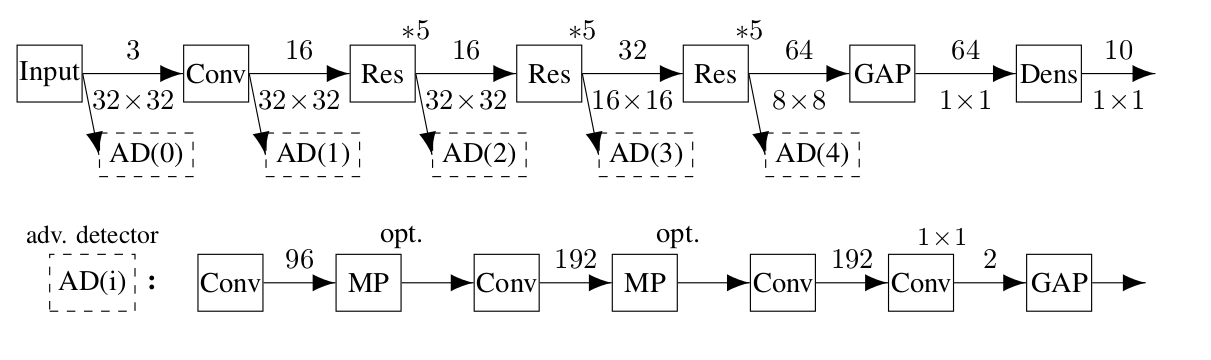
\includegraphics[scale=0.30]{detection}
                \caption{Metzen \textit{et al.} (Ref. ) used a ResNet as original classifier, plus dections is made thanks to many interleaving detectors
                between each residual block. Each detector is implemented as a DNN that learns how to spot the presence
                of an attack by looking at the activations layer's distributions during training.}
                \label{fig:detection}
            \end{figure}

            In case of a supervised detection mechanism, we want to augment our data with labelled samples crafted with known
            attacks and build a binary classifier which is able to distinguish between vanilla and altered inputs. The key 
            point here is then to test such classifier on new, previously unseen attacks and check how well it adapts.  
            Papernot er al. in (Ref. On the (statistical) and Feinman et al. in (Ref. Detecting adversarial samples from artifacts)
            developed two sophisticated early versions of such detection type, but both failed to detect ad-hoc CW (Ref. ) attacks on CIFAR-10.
            Better results against CW were achieved  by Metzen \textit{et al.} (Ref. On Detecting Adversarial Perturbations), whose method
            works by feeding DNN layer's activations as features to a detector Fig. \ref{fig:detection}. In particular, in detecting CW on CIFAR-10
            were 81\% TPR and 28\% of FPR. However they reported that they were not able to generalize well 
            to other attacks, which shows a limitation of their method (or even to any supervised detection?), 
            that is, to likely overfit on the attacks used for training (Ref. BYpassing 10 Detection Methods).

            In literature, as well as supervised detection mechanisms, there have been also many 
            detection classifier which were not trained on adversarial examples, thus performing sort of unsupervised detection.
            They instead rely on explicit null hypothesis and statistical models to work, such as based on PCA (Ref. Early methods for
            detecting adversarial images), which again however showed uneffective against CW for CIFAR-10, (Ref. Towards open set
            deep networks), or analyzing the joint density of a DNN's layer feature vector (Ref. Detecting adversarial samples from artifacts).
            In particular, based on the latter, recently Miller \textit{er al.} in (Ref. Anomaly
            detection of attacks (ADA) on DNN classifiers at TEST TIME,) managed to develop the current state-of-the-art for detection
            methods as stated in (Ref. 2020 Survey on Defenses.). The description of such method is however quite involving and esulate from
            the objective of this thesis.
            
            
            \subsection{Robust Optimization}

                What if we train a DNN such that, together with minimizing the loss we also
                train to minimize the effects of adversarial examples? That is, how do we go and train
                a DNN which performs well on both clean and perturbed inputs? As it turns out, to perform
                such training, we need to solve the following, intuitive, min-max problem:
                \begin{equation}
                    \label{robopt}
                    \underset{\theta}{\operatorname{min}} \frac{1}{|S|} \sum_{x, y \in S} \max _{\delta \in \Delta} \operatorname{LS}\left(f_{\theta}(x+\delta), y\right),
                \end{equation}
                that goes under the name of \textit{Robust Optimization}.
                
                The order of the optimizations is important here. The maximization is inside the minimization, this
                intuitively means that we are training in a way that: even if the adversary knows the 
                parameters of the model $\theta$ and performs his best attack over it, we contrast
                its effects by minimizing the empirical risk on such attack, as with standard training.
                Moreover, notice that we just learned how to compute strong attacks e.g. with randomized PGD, thus we
                can already go and implement Robust Optimization, which, to be precise, it is mostly reffered as \textit{Adversarial
                Learning} (AL) when we approximate the solution instead of computing it exactly (Ref. https://arxiv.org/pdf/2007.00753.pdf ).

                In practice, even if the training is performed employing random PGD to compute the inner maximization,
                i.e., a very specific form of attack, it does generalize well to other attacks (Ref. Madry article in Robust Optimization), 
                provided that we consider attacks under the same metric. Indeed, there is no real guarantee that AL
                done under, say, $\|\cdot\|_2$ will result in a model also robust against $\|\cdot\|_{\infty}$ based 
                attacks. To achive defenses against multiple metrics, we need to incorporate multiple attacks under the inner maximization,
                however, as previously discussed, characterizing a priori every possible metric of perturbation seem to be 
                a difficult task, hence the complexity of devising an universal defense mechanism.

                The main drawback with AL, which is so far regarderd as the most effective method developed agains adversarial
                Examples (Ref. ), is its computational demand. Indeed, due to the double optimization that needs to be
                computed for each weight update on each sample, it requires a lot of resources, especially when it comes
                to large networks and large datasets. For this reason, lately, different works tried to takle the
                problem of speeding-up AL, proposing approximations and variations of it (Ref. Free AL)(Ref. Fast is better than free).

                
            
            \subsection{Provable Robustness}

            Provable defenses try to theoretically find certificates in distances or probabilities to certify the robustness of DNNs.
            Can \ref{robopt} be exactly solved? Namely, can we find the optimal set of weights such to minimize 
            the error on Adversarial Examples? This is in principle a legitimate question to ask, and several 
            strategies have been proposed, all of which somehow works providing an upperbound for the inner maximization.
            In this way, defined the threat model, we can make stronfer statements about the guarantees for the defense.
            If we rewrite the innner maximization as the following adversarial loss:
            \begin{equation}
                \mathcal{L}_{a d v}=\max _{\sigma \in \Delta}\left\{\max _{i \neq y} f_{\theta}(x)\left(x + \delta\right)_{i}-f_{\theta}(x)\left(x + \delta\right)_{y}\right\},
            \end{equation}
            then, if we are capable to define an always larger certificate $ C(x, f_{\theta}) > \mathcal{L}_{a d v}$ and prove
            \begin{equation}
                C(x, f_{\theta}) < 0
            \end{equation}
            under certain constraints, the we are sure that, under the same constraints, e.g., on the bound of 
            the perturbation, our model will always predict the correct class. Employing this argument,
            [112] transforms the problem into a linear programming problem and [111] derives the certificate using
            semidefinite programming.
            
            Differently, !!Pippo!! \textit{et al.} (Ref. Intriguing) pointed out the relation that exists 
            between the so called \textit{Lipischitz Constant} and the sensitivity of the network 
            with respect to input perturbations. Specifically, denote $f_{\theta}(x) = f_{\theta_L}(f_{\theta_{L-1}}(\cdots (f_{\theta_{1}}(x))\cdots)) $
            then the Lipschitz Constant of  $f_{\theta_i}(x)$ with respect to the norm $ \|\cdot\|_p $ is defined to be
            the smallest $L_i$ such that, for any $x, r \in \mathcal{X}$:
            \begin{equation}
                \label{LC}
                \left\|f_{\theta_i}\left(x \right)-f_{\theta_i}\left(x+r\right)\right\|_p \leq L_{i}\|r\|_p .
            \end{equation}
            Notice how $L_i$ by definition is an upperbound for the sensitivity of layer $i$ with respect
            to any perturbation $r$. Following the composition property of the
            Lipschitz Constant, the overall network Lipschitz Constant will be, the smallest $L$ such that:
            \begin{equation}
                \left\|f_{\theta}\left(x \right)-f_{\theta}\left(x+r\right)\right\|_p \leq L\|r\|_p,
            \end{equation}
            where $L=\prod_{i=1}^{L} L_{i}$. It is important to note how this is only an upperbound, thus a conservative
            measure of the possible unstability of the network. For this reason, no conclusion about the existence of 
            Adversarial Examples can be derived even from large Lipischitz Constants. We are however guaranteed 
            that for very small Lipischitz Constants no Adversarial Example will exist. This is the idea behind 
            many regularization techniques that seek to penalize Lipschitz bounds on networks's components as 
            in (Ref. ) (Ref. )

            Many other approaches try to provide certificates such as \textit{Randomized Smoothing}, \textit{estimation of the lower bound} (Ref. https://arxiv.org/pdf/2007.00753.pdf)
            . However, provable Robustness struggles to scale up to real-world applications
            due to the complexity of computing such bounds that are usually based on generally intractable methods or ad-hoc methods.





    \chapter{Non-Parametric Activation Functions}

    As anticipated shortly in the section concerning Activation Functions, it is possible to increase the flexibility of a Neural Network replacing a fixed activation function with a parametrized, differentible, non-linear function.
    These transformations can in fact be trained along with the remaining weights of the network allowing each neuron to model its own optimal shape.

    Scardapane \textit{et al.} in (Ref. KafNets) grouped together different works on such activation functions distinguishing, on the high level, between the number of parameters they involve in their formualtions.
    In particular, whenever we add a constant number of weights to a fixed activation function, authors say we are dealing with 'parametric activation functions'. Some examples of this class of functions are: the \textit{Generalized Hyperbolic Tangent} (Ref. )
    , a parametric Leaky ReLU introuced by He \textit{et al.} (Ref. ) or the more flexible S-shaped Relu (SReLU) (Ref.  Jin et al.):
    \begin{equation}
        \label{srelu}
        \operatorname{SReLU}(x)=\left\{\begin{array}{ll}
            t^{r}+a^{r}\left(x-t^{r}\right) & \text { if } x \geq t^{r} \\
            x & \text { if } t^{r}>x>t^{l} \\
            t^{l}+a^{l}\left(x-t^{l}\right) & \text { otherwise }
            \end{array}\right.
            ,
    \end{equation}
    parametrized by $\{t^l,a^l,t^r,a^r\}$. Depending on the values assumed by the left ($l$) and right ($r$) parameters, SReLU can assume both convex and non convex shapes.

    What happens if we give to activation functions greater modeling capabilities, what if we allow them to model any continuous segment? This question is instead addressed by the class of 'non-parametric activation functions'. These methods,
    usually introduce a further global hyper-parameter, allowing to balance the number of parameters that can in principle grow without a bound, hence the name.

    In this section, we give an overview of three early proposals, describing the general idea and some of the drawbacks, if any. After that, we focus on a more recent kind of non-trainable activations called kernel-based activation Functions
    (KAFs), highlighting their properties and experimental results.

    \section{Adaptive Piece-Wise Linear Activation Functions}
            Introduced in (Ref. Agostinelli et al 2014), APL generalize the SReLU \ref{srelu} activation function summing up $S$ parametrized linear segments that are
            learned under the constraint that the resulting function is continuous:
            \begin{equation}
                \operatorname{APL}(x) = max \{0, x\} + \sum_{i=1}^{S} a_{i} \max \left\{0,-x+b_{i}\right\},
            \end{equation}
            where $S$ is a user-defined value and $a_i$s the parameters to learn. APL adds $2S$ new parameters per neuron i.e. introducing a linear number of parameters to the overall network, which is often feasable.
            APL cannot, however, model or approximate all piece-wise linear functions, but only saturating ones. Moreover, APLs introduce $S$ non-differentiable points which may harm backpropagation.
    \section{Spline Activation Functions}
    If we want an activation function capable of interpolating $S$ given points, we can devise the following polynomial interpolation:
    \begin{equation}
        \sigma(x) = \sum_{i=0}^{S} a_{i} x^{i},
    \end{equation}
    where we actually going to learn $S+1$ coefficients to pass through the desired $S$ points. Thus, in theory, we can at least approximate, by means of
    a sufficiently large $S$, any smooth function albeit in practice, due to the global effect that any parameter has on the global shape, such approximation
    is hard. Moreover, $x^i$ can easily grow too much and encounter numerical problems.
    
    Instead of using polynomial interpolation, (Ref. ) proposed the use of \textit{spline interpolation} that results in the so called spline activation functions (SAFs).
    Let $\{ x_1, x_2, \cdots, x_S \}$ be an equally spaced sampling of real values, symmetric to the origin and with step size $\Delta x$ and call \textit{knots}
    the corresponding y-valules $\{\operatorname{SAF}(x_i)\}^S_{i=0}$ . Denote $u=\frac{t}{\Delta x}-\left\lfloor\frac{t}{\Delta x}\right\rfloor$ to be the normalized ascissa 
    value between to consecutive knots when the activation is $t$. Finally, we can define SAF at $t$:
    \begin{equation}
        \label{saf}
        \operatorname{SAF}(t)=\mathbf{u}^{T} \mathbf{B} \mathbf{q}_{k},
    \end{equation}
    where $\mathbf{u}=\left[u^{P}, u^{P-1}, \ldots, u^{1}, 1\right]^{T}$, $P$ is a user-defined value (usually chosen to be 3), $\mathbf{q}_{k}$ the vector composed by
    the closest knot to $t$ and the $P$ rightmost neighbors knots and $\mathbf{B} \in \mathbb{R}^{(P+1) \times(P+1)}$ the \textit{spline basis}. Different basis give 
    rise to different interpolation schemes (Ref. ).
    
    Good news with SAFs is that each knot has only a local effect on the overall shape. Therefore, with respect to the initialized knots, their training allows for faster and better convergence
    to the optimal. Moreover, as with polynomial interpolation, SAFs can in principle approximate any smooth function. A drawback, however, 
    comparing to ALF, is that regularization techniques cannot be explicitly implemented.
    \section{Maxout Functions}
    One slightly different non-parametric activation function, is given by the introduction of a whole new layer called \textit{maxout function}. With maxout, we compute $K$ different dot products
    on each neuron and then take the maximum:
    \begin{equation}
        \operatorname{maxout}(x) = \max \{  W_i^Tx + b_i \}_{i=1}^K .
    \end{equation}
    A DNN wich employs maxout functions as non-linearities is called \textit{Maxout Network} (Ref. ). As for APL, maxout introduces several points of non-differentiability and usually requires 
    \begin{figure}[!h]
        \centering
        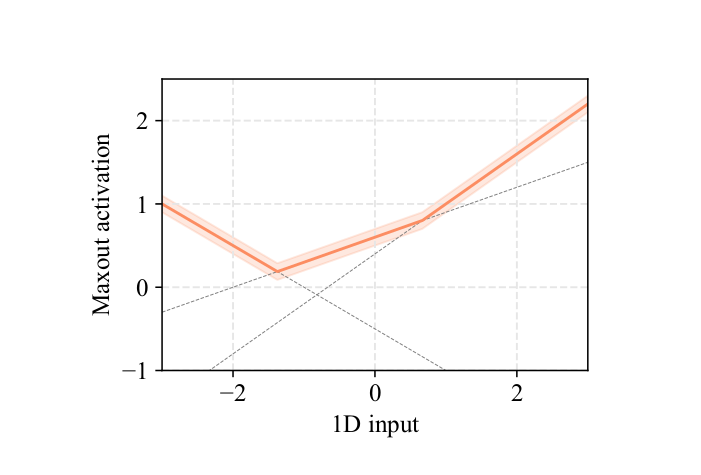
\includegraphics[width=0.6\textwidth]{maxout}
        \caption{A maxout function with a one-dimensional input and K = 3. The
        three linear dot products are shown with light gray, while the max and thus resulting activation is shown
        in shaded red. Source: (Ref. )}
        \label{fig:maxout}
    \end{figure}
    more parameters than previous approaches, as we scale by a factor of $K$ the number of weights inside the net. Furthermore, maxout can only generate convex shapes and 
    we lose the ability of plotting the activation function, except for input up to three-dimensional Fig. \ref{fig:maxout}.
    Different variations aim to solve the smoothness problem for Maxout Networks (Ref. ) (Ref. ). 

    \section{Kernel-Based Activation Functions}
    Introduced in (Ref. Kafnets), kernel-based activation functions (KAFs) is a class of non-parametric activation functions that leverage kernel expansions to adapt the shape on a per-neuron basis.
    Let $D$ be a user-defined positive integer, then a KAF acting on activation $x \in \mathbb{R} $ has the following form:
    \begin{equation}
        \operatorname{KAF} (x) = \sum_{i=1}^{D} \alpha_{i} \kappa\left(x, d_{i}\right),
    \end{equation}
    where $\{ \alpha_i\}_{i=1}^D $ are the usual parameters to adapt, called \textit{mixing coefficients}, $\kappa \colon \mathbb{R} \times \mathbb{R} \to \mathbb{R}$ is a 1D kernel method (Ref. )   
    and $\{ d_i\}_{i=1}^D $ the kernel's dictionary elements. Dictionary elements are usually sampled from training data, but in case of activation functions 
    this would tie the size of the expansion $D$ to the specific dataset used. Since generality is preferred, KAFs use fixed dictionary elements by selecting
    $D$ equally spaced points on the x-axis centered at 0 with step size $\Delta$, similary to SAFs. In particular, there is a vast literature on kernel methods with fixed dictionary elements (Ref. Snelson and Ghahramani, 2006).
    A Neural Network that makes use of KAFs is called \textit{Kafnet}.

    To allow for better optimization with Gradient Descent we want the kernel $\kappa(\cdot, \cdot)$ to be positive semi-definite and thus convex, i.e., for any choice of 
    $\{ \alpha_i\}_{i=1}^D $ and $\{ d_i\}_{i=1}^D $ we have:
    \begin{equation}
        \sum_{i=1}^{D} \sum_{j=1}^{D} \alpha_{i} \alpha_{j} \kappa\left(d_{i}, d_{j}\right) \geq 0 .
    \end{equation}
    As for which kernel method one should use, to perform our experiments in the following chapters, we will stick to the original paper and use the 1-dimenstional \textit{Gaussian kernel}:
    \begin{equation}
        \kappa\left(x, d_{i}\right)=\exp \left\{-\gamma\left(x-d_{i}\right)^{2}\right\},
    \end{equation}
    where the normalization term $\gamma$ is called \textit{kernel bandwidth} and is empirically chosen to be $ \gamma = \frac{1}{6 \cdot \Delta^2} $.
    The Gaussian kernel is easy to implement using vectorization libraries and quite cheap to compute provided that the dimensions don't grow too large. Moreover, 
    concerning the backward pass, KAFs have pretty straightforward derivatives as well:
    \begin{equation}
        \frac{\partial g(x)}{\partial \alpha_{i}}=\kappa\left(x, d_{i}\right),
    \end{equation}
    \begin{equation}
        \frac{\partial g(x)}{\partial x}=\sum_{i=1}^{D} \alpha_{i} \frac{\partial \kappa\left(x, d_{i}\right)}{\partial x}.
    \end{equation}
    Additionally, employing the Gaussian kernel has two more benefits: first, it allows for locality effects of parameters and second, the resulting (Gaussian) KAF
    is an universal approximator for continuous segments (Ref. Micchelli et al., 2006).

    The mixing coefficients can either be initialized randomly from a normal distribution, giving no direction yet complete freedom in the trend that the modeled shape
    should follow Fig. \ref{fig:rand}, or, on the contrary, we can initialize mixing coefficients such that the KAF will start with an interpolation of any given function $f$
    Fig. \ref{fig:ridge}. Let $\mathbf{t} = (t_1, t_2, \cdots, t_D) $ be the set of values assumed by $f$ when acting on dictionary elements i.e. $\mathbf{t} = (f(d_1), f(d_2), \cdots, f(d_D)) $.
    We can then initialize the mixing coefficients in the following way:
    \begin{equation}
        \mathbf{\alpha} = \left(K  + \epsilon I \right)^{-1} \mathbf{t}
    \end{equation}
    where $K \in \mathbb{R}^{D,D}$ is the kernel matrix with $K_{i,j} = \kappa(d_i, d_j)$ entries, and we add a diagonal term $\epsilon > 0$ to avoid degenerate 
    solutions. To constrain and regularize the learned parameters, contrary to SAFs, KAFs also allow the use of common regularization techniques.
    \begin{figure}
        \centering
        \begin{minipage}{0.45\textwidth}
            \centering
            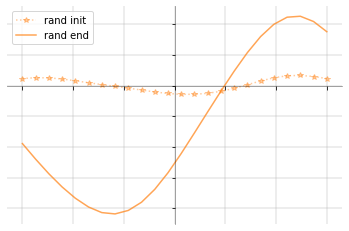
\includegraphics[width=0.9\textwidth]{randridge.png} % first figure itself
            \caption{The shape of a KAF with randomly initialized coefficients is shown in light-starred orange. The final learned shape of the same KAF after 
            training is shown with a continuous orange line. Notice the strong difference between the two functions and how the final one resembles a shifted
            tanh.}
            \label{fig:rand}
        \end{minipage}\hfill
        \begin{minipage}{0.45\textwidth}
            \centering
            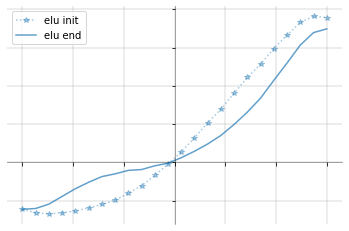
\includegraphics[width=0.9\textwidth]{eluridge.png} % second figure itself
            \caption{The shape of a KAF with coefficients initialized through ridge regression to approximate the ELU function is shown in light-starred blue.
            The final shape after training is shown with a continuous blue line. Notice how the difference between the two is less evident comparing to randomly 
            initialized KAF (left). Both KAFs (left and right) were trained on the same neuron for the \textit{MNIST} dataset using 5 epochs and same overall settings.  }
            \label{fig:ridge}
        \end{minipage}
    \end{figure}
    It is also worth mention that we can improve the flexibility of KAFs by letting the network adapt, along with mixing coefficients, both the dictionary elements
    and the bandwidth. This further level of flexibility can indeed help reach better performances as will be shown in the Evaluation chapter.

    In (Ref. KafNets) authors performed different experiments to assess the performances of the proposed KAFs.
    It turned out that KAFs managed to improve the results obtained with fixed activation functions over several benchmarks ranging from simple datasets 
    like the \textit{Sensorless} dataset (Ref. ) to larger ones such as \textit{SUSY} (Ref. SUSY dataset), testing on shallow feedforward Neural Networks
    as well as deeper CNNs architectures and for both supervised and unsupervised tasks. A summary of the reported results is given in Table \ref{tab:scardapanekafexp}.  
    
    \begin{table}
        \begin{tabular}{ |p{1.5cm}||p{2cm}|p{1.6cm}|p{2.3cm}|p{2.5cm}|p{2.8cm}|  }
            \hline
            \multicolumn{6}{|c|}{\textit{Scardapane et al. KAF Experiments}} \\
            \hline
            \textbf{Dataset} & \textbf{Design} & \textbf{Metric} & \textbf{Fixed AF}& \textbf{Param. AF} & \textbf{Non-param. AF}\\
            \hline
            \hline
            Sensorless & FNN$^*$  &Accuracy&tanh:99.18\% &PReLU:99.30\% & \underline{ KAF:99.80\% } \\
            \hline
            SUSY&   FNN$^{**} $ &AUC&ReLU:0.8739 & PReLU: 0.8748&Maxout:0.8744 APL:0.8757 \underline{KAF:0.8758} \\
            \hline
            CIFAR10 & CNN$^{***}$ &Accuracy&ELU:78\% & \textit{n.a.} & \underline{ELUKAF:83\%} \\
            \hline
        \end{tabular}
        \caption{Each row summarize the results obtained using different activation functions on a specific task. 
        Underlined entries stand for best result achieved.
        $^*$: feedforward neural networks with 3 hidden layers of 100 neurons are used for fixed or parametric activation functions whilst a single hidden layer is used 
        for KAF activation function.
        $^{**}$: feedforward neural networks with 5 hidden layers and 300 neurons each for fixed or parametric activation functions whilst 2 hidden layers with the same
        number of neurons for non-parametric activation functions \\
        $^{***}$: CNNs made by stacking 5 convolutional blocks, each composed by (a) a convolutive layer with 150 filters, with a
        filter size of 5 × 5 and a stride of 1; (b) a max-pooling operation over 3 × 3
        windows with stride of 2; (c) a dropout layer with probability of 0.25. See the original article for a full description of the architectures, hyperparams and training
        settings.}
        \label{tab:scardapanekafexp}
    \end{table}
       
    
\part{Robustness of Kafnets}

    \chapter{Related Works}

    Among t
       
    \section{K-Winners Take All}
    In (Ref. ENHANCING ADVERSARIAL DEFENSE BY k-W INNERS-TAKE-ALL), Xiao \textit{et al.} advocate the use of a $C^0$-discontinuous activation function, called
    \textit{k-Winners-Take-All} (k-WTA) activation, to improve, with no substantial overhead, the robustness of a neural network against gradient-based attacks such as PGD.
    k-WTAs work by acting on the whole layer $\mathbf{y}$, similarly to maxout, but in this case they filter the input retaining the k-largest values and deactivating to 0 the remaining ones.
    More formally, a k-WTA acting on an input vector of neurons $\mathbf{y} \in \mathbb{R}^{n}$ is a function $\phi_k(y) : \mathbb{R}^n \to \mathbb{R}^n$ such that:
    \begin{equation}
        \phi_k(\mathbf{y})_j = \left\{\begin{array}{ll}
            y_{j}, & y_{j} \in\{k \text { largest elements of } \boldsymbol{y}\} \\
            0, & \text { Otherwise. }
            \end{array}\right. 
    \end{equation}
    where $\phi_k(\mathbf{y})_j$ denotes the j-th element of the output. Notice how $\phi_k(\mathbf{y})$ is effectively 
    parametrized by $k$ but it cannot be regarded as a parametric activation function since $k$ is user defined and not
    differentiable. Moreover, since it is likely to have layers with different shapes inside a net, we use the \textit{ratio $\lambda$}
    of the number of neurons of each layer to compute the correct $k$, simply as $k = \lambda \cdot |layer|$.

    K-WTAs foster robustness by making the computation of the gradient $\nabla_x f_{\theta}(x)$ \textit{undefined}.
    Loosely speaking, this is achieved thanks to densely distributed discontinuities in the space of $x$. Indeed, this implies that,
    with very high probability, any perturbation moving $x$ to it's neighbourhood will move over a non-differentiable spot Fig. \ref{fig:kwta}.
    in the adversary objective, making gradient-based search unfeasable. The meticolous reader may at this point start to wonder
    how is thus even possible to perform training with such discontinuous functions. However, it turns out that the gradient 
    with respect to the weights $\nabla_w f_{\theta}(x)$ is discontiuous but in a sparser way, presumably beacuse the parameter 
    space where $w$ leaves is much larger than the input space, allowing the training to succeed. To gain a better understanding
    of what is going on, the paper provides also a theoretical framework in which both the dense discontinuities and the trainability 
    can be explained. Since k-WTAs are only marginally used in the following parts of this thesis, we will not go in the details
    of such proofs.

    \begin{figure}[h]
        \centering
        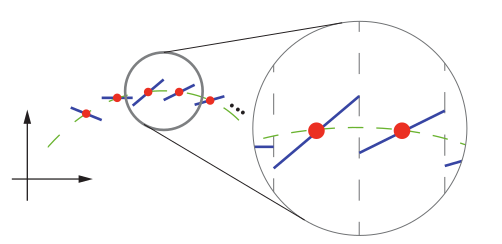
\includegraphics[width=0.6\textwidth]{kwta}
        \caption{A plot of a 1-dimensional k-WTA interpolating a curve. As stressed by the figure, k-WTAs are piece-wise linar functions where points of non-differentiability are 
        very much densely distributed. Any small change in the input results in an abrupt change in the function's value. Source: (Ref. )}
        \label{fig:kwta}
    \end{figure}
    
    Authors claim substantial improvements in the robustness of this defense against white-box attacks. Specifically, they were 
    able to evaluate a ResNet-18 against PGD, C\&W (Ref. ) and DeepFool (Ref. ) attacks, training both classically and with AL \ref{robopt}.
    Using CIFAR10 for the dataset, ResNet-18 with ReLUs achieved 0\% and 43.6\% accuracy under the most effective attack,
    respectively with standard and adversarial training. On the other hand, when k-WTAs were used, the same network improved to
    13.1\% with standard training and 50.7\% with AL.

    In a recent work (Ref. ), Carlini \textit{et al.} highlighted fundamentals flaws in the defense that was just claimed for k-WTAs.
    Authors were in fact capable of showing how this method falls within a broader category of attacks, known as gradient-masking
    defense methods (Ref. survey 2), which are already known in literature to be vulnerable.
    It is nevertheless true that, for unadaptive and straightforward implementations of current gradient-based attacks, k-WTAs
    still provide a fair protection, especially when the networks is adversarially trained. For this reason, in the following chapters
    we will make use of k-WTAs (for which we give a novel implementation in \textit{TensorFlow2}), as a benchmark for our evaluations.

    \section{Smooth Adversarial Training}

    The current wisdom among researchers, suggests that there probably is a fundamental trade-off between accuracy and robustness that we must deal with
    (Ref. There is no free lunch in adversarial robustness). That is, improving the resiliency of a model against adversarial examples will almost certainly 
    result in a less accurate model. In particular, whenever an effective technique to improve the robustness is found, it almost always coincides with the method harming
    the model performances (Ref. On the convergence and robustness of adversarial training) (Ref. Max-margin adversarial training) (Ref. 
    Theoretically principled trade-off between robustness and accuracy).
    
    To prevent from performance decay, one feasable (but expensive) strategy is to increase the size of the network by making it either deeper and/or wider (Ref. Intriguing Properties of NNs at scale.).
    It seems nevertheless reasonable to believe that there could be other ways that would allows us to build more robust networks without 
    sacrificing in neither accuracy nor resources. That is exaclty what was recently reported by Xie \textit{et al.} in (Ref. Smooth Adversarial Training), where authors 
    found a way to consistently improve robustness over different tasks, without giving up any other property of the model. Specifically, they found that,
    it is sufficient to prefer and adopt smooth activation functions over non-smooth ones, like the everywhere present ReLUs, to achieve 
    better results in AL straightaway.

    The rationale behind adopting smooth activation functions, i.e., non-linear functions that are continuous in their first derivative, lies in the 
    observation that, during AL, we are computing many times the gradients of the network that are normally required during standard training. Specifically,
    in addition to compute gradients to update the network's parameters, adversarial learning also needs gradients computation for generating training 
    adversarial samples. Moreover, the presence of non differentiable points and abrupt changes in the gradient's values during backpropagation, may 
    prevent from generating sufficiently strong adversarial samples. This particularly holds true in the case of ReLUs, where the gradient lacks of flexibility 
    and gets a severe jump in the origin Fig. \ref{fig:smoothaf}. 

    \begin{figure}[h]
        \centering
        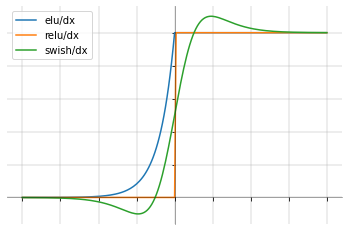
\includegraphics[width=0.45\textwidth]{smothaf.png}
        \caption{Plot of the first derivative for ReLU, ELU and Swish activations. Except for the rectified linear unit, both the ELU and Swish have continuous
        derivative.}
        \label{fig:smoothaf}
    \end{figure}

    To test their hypothesis, Xie et al. evaluated a ResNet50 on ImageNet for different AL runs, by switching activation function after each training. For their experiment,
    parametrized \textit{Softplus} (Ref. ), Swish, \textit{GELU} (Ref. ) and ELU were used as smooth activations, whereas ReLU for the baseline. Notice that,
    for the case of ELU, the parameter $\alpha$ \ref{elu} should be set equal to 1 in order to avoid the gradient being undefined at the origin. Compared to the 
    baseline, all smooth activation functions substantially boosted robustness while keeping the accuracy nearly unchanged. In particular, any smooth activation 
    function at least improved robustness by a factor of $5.7\%$. 
    \begin{figure}[t]
        \centering
        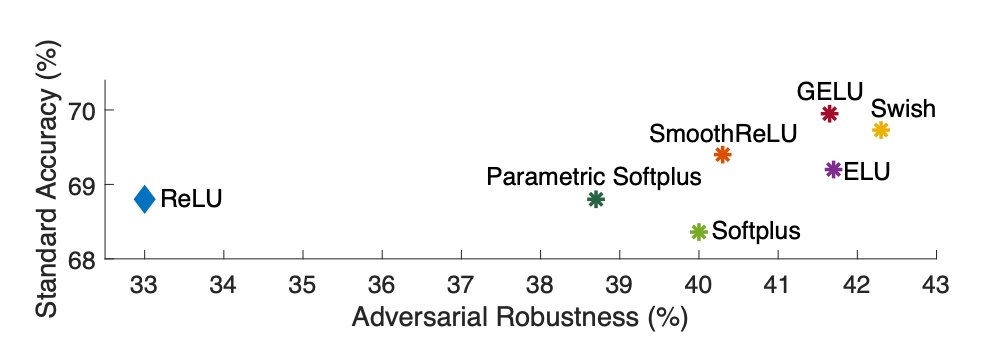
\includegraphics[width=0.75\textwidth]{smoothresults}
        \caption{Compared to ReLU, all smooth activation functions showed a significant increase in robustness
        while some even improved accuracy. In the original work, 2 others smooth activation functions were used, namely 
        SmoothReLU and Softplus. We did not include them since they are not commonly used in practice. Source: (Ref. Adversarlial Smoothness)}
        \label{fig:smoothresults}
    \end{figure}
    Best results were achieved with Swish, which enabled
    ResNet50 to achieve $42.3\%$ robustness and $69.7\%$ standard accuracy as shown 
    in Fig. \ref{fig:smoothresults}

    To test further the issue with ReLU and generalize the smoothness conjecture, another 
    experiment was made targetting ELUs. As we said, when we set the parameter $\alpha$ to be different to 
    1, the function becomes non-differentiable in the origin, with the gradient
    abruption increasing for larger values of $\alpha$. With no surprise, if we perform the same evaluation with no change in the settings
    except for equipping the network with non-smooth ELUs,
    we observe that the adversarial robustness is highly dependent on the value of $\alpha$. 
    The highest robustness is achieved when the function is smooth while for all other choices of 
    $\alpha$ the robustness monotonically decreases when we gradually approache $\alpha = 2.0$. 
    In particular, with $\alpha$ being $2.0$, robustness drops to $33.2\%$, that is, $7.9\%$ lower than that of smooth ELU. 
    The observed results are consistent with previous conclusions on ReLU: non-smooth activation functions significantly
    weaken adversarial training.

    From a broader perspective, the work on smooth activation functions might
    hints towards the draft of a more general design principle, which is that,
    architectural smoothness might play an essential role in enhancing 
    adversarial rbustness, at least for what concerns defenses against 
    gradient-based attacks.

    With a combination of lessons just learned from both Xiao et al. and
    Xie et al., the focus of the following chapters will then be on the evaluation
    of a novel kind of activation functions. Functions that we believe might have 
    , by laveraging, among other properties, strong smoothness
    and flexibility, the potential of surpassing both k-WTAs and Swish 
    for what concerns robustness and, in particular, the trade-off
    between accuracy and robustness. Distinguished activation functions that 
    satifsy such prerequisites are the previously introduced non-parametric 
    kernel-based activation functions (KAFs). 



\chapter{Solution Approach}
 
    To start experiment novel architecuters or training techniques in practice, they need first to be implemented. In our case, we have chosen to use
    Python with TensorFlow2 library to craft DL methods. In this way, relying on the \textit{Keras} backend, it is possible to describe complex activation functions, in which for instance the output depends on the input layer size, as for both k-WTAs and KAFs. To this end we implemented them inheriting from the 
    \textit{tf.keras.layers.Layer} class. The code that implements both activation functions is located in \textit{activationsf.py}.
     

    \section{KAFs May Be Good Candidates}

        Once the code is done, we can begin and perform some early evaluations. As a first thing, we reasonably chose to test the robustness of simple neural 
        networks and in particular, we can already try to understand if there is any meaningful difference when we change activation functions.

        The light first-developed model is made of few parameters, to conduct quick experiments and perhaps find an initial direction to follow. The network 
        is composed by two convolutional blocks, each of which holding two convolutional layers followed by batch normalization. After those two convolutions we 
        halve the dimensions with a maxPooling and then apply regularization with Dropout. In the first block we use 32 filters, in the second 64, each with window 
        size 3. Finally, a global average pooling is used followed by a fully-connected layers with 128 units which is in charge of computing the output layer.
        The dataset used, and the only one that we will be using for each evaluation, is CIFAR10. The code where such networks are built and trained can be found in 
        \textit{light\_models.ipynb}.

        Respectively, using ReLU, k-WTA and KAFs (with randomly initialized mixing coeffiecients and D=20) and using Adam optimizer, we obtained 77.96\%, 65.33\%
        and 68.80\% standard accuracy. After that, we are ready to see how such trained nets behave against adversarial examples. Following the settings of 
        (Ref. kWTA), a $PGD$ attack is crafted under the $L_{\infty}$ metric, with perturbation size $\epsilon = 0.031$, steps size $0.003$ and 40 random 
        restarts. Importantly, we only attack 1000 random samples taken from the test set, since, due to resources limitations we were not capable of computing 
        the attack on the whole network in reasonable time and, moreover, because we only wanted to a rough estimate to begin with. To actually implement such attacks we 
        will use the \textit{Adversarial Robustness Toolbox} (ART) from IBM (Ref. ? should i cite this?).


        

    \section{Fast is Better than Free Adversarial Training}

        Adversarial training (Madry et al.) and current methods to improve the efficiency (Fast is better than free)


\chapter{Evaluation}

    \section{VGG Inspired Architectures Results}

    \section{Explofing Gradients with KafNets}

        The exploding gradients problem with KafResNet, why is it happening? (still to clarify)

    \section{ResNet20 Inspired Architectures Results}


\chapter{Future Works}

    Different Kernels, resolve the exploding gradient problem and scale to ImageNet
    Perform more adaptive attacks to assess the robustness of kafresnets as is the current standard (Carlini et al.)


\chapter{Conclusions}

    This thesis tries to add to the bag of evidences in literature that smoother architectures might benefit improvements in adversarial resiliency
    
    
\appendix


\backmatter
% bibliography
%\cleardoublepage
%\phantomsection
%\bibliographystyle{sapthesis} % BibTeX style
%\bibliography{bibliography} % BibTeX database without .bib extension

\end{document}
